\documentclass[11pt,a4paper]{article}

% --- Packages ---
\usepackage[utf8]{inputenc}
\usepackage[margin=1in]{geometry}
\usepackage{amsmath,amssymb,amsfonts}
\usepackage{booktabs}
\usepackage{tabularx}
\usepackage{graphicx}
\usepackage{xcolor}
\usepackage{microtype}
\usepackage{caption}
\usepackage{subcaption}
\usepackage{fancyhdr}
\usepackage{titlesec}
\usepackage{setspace}
\usepackage{hyperref}

% --- Hyperref Setup ---
\hypersetup{
    colorlinks=true,
    linkcolor=blue!70!black,
    citecolor=blue!70!black,
    urlcolor=blue!70!black
}

% --- Header and Footer Styling ---
\pagestyle{fancy}
\fancyhf{}
\fancyhead[L]{\small Machine Learning Project: Air Quality Sensor Calibration}
\fancyhead[R]{\small Final Research Report}
\fancyfoot[C]{\thepage}
\renewcommand{\headrulewidth}{0.4pt}
\renewcommand{\footrulewidth}{0.4pt}

% --- Section Heading Formatting ---
\titleformat{\section}{\large\bfseries\color{blue!60!black}}{\thesection.}{0.5em}{}
\titleformat{\subsection}{\normalsize\bfseries\color{blue!40!black}}{\thesubsection}{0.5em}{}
\titleformat{\subsubsection}{\normalsize\bfseries\itshape\color{blue!30!black}}{\thesubsubsection}{0.5em}{}

% --- Line Spacing ---
\setstretch{1.12}

\begin{document}

% =========================================================================
% TITLE BLOCK
% =========================================================================
\begin{center}
    {\LARGE \textbf{\color{blue!60!black} COMPARATIVE ANALYSIS OF MACHINE-LEARNING ALGORITHMS FOR LOW-COST AIR QUALITY SENSOR CALIBRATION UNDER HIGH-HUMIDITY AND POLLUTION EXTREMES}} \\[1.2em]
    {\large \textbf{Research Project Report}} \\[0.4em]
    {\normalsize \textit{Submitted as part of the Machine Learning Project Coursework}} \\[0.4em]
    {\small \textbf{Focus:} Machine Learning Algorithms (Random Forest, Gradient Boosted Trees / XGBoost, and Support Vector Regression)} \\[0.2em]
    {\small \textbf{Datasets:} PurpleAir India Co-location Network \& Q-SCALE Turin Italy Benchmark} \\[0.2em]
    {\small \textit{Prepared for Academic Evaluation and Peer Review}} \\[1.5em]
    \rule{\textwidth}{0.8pt}
\end{center}

% =========================================================================
% ABSTRACT & KEYWORDS
% =========================================================================
\begin{abstract}
Low-cost optical particulate matter ($\text{PM}_{2.5}$) monitors allow dense community air-quality networks, but their raw readings suffer from significant baseline drift, particle density mismatches, and severe aerosol hygroscopic growth (water uptake) when ambient relative humidity exceeds 70\%. Standard static corrections, including the US EPA nationwide linear equation, cannot capture non-linear humidity deliquescence surges and seasonal pollution inversions. This report compares three machine-learning algorithms---Random Forest (RF), Gradient Boosted Decision Trees (GBDT / XGBoost equivalent) and Support Vector Regression (SVR with RBF kernel)---alongside Multiple Linear Regression (MLR) and raw uncalibrated sensor baselines across two independent datasets. Dataset 1 comprises multi-site PurpleAir PA-II co-location records from India (Delhi, Hamirpur and Bengaluru; 25,829 valid hourly records; $\text{PM}_{2.5}$ range 4 to 480~$\mu\text{g}/\text{m}^3$) paired against Met One BAM 1020/1022 regulatory monitors. Dataset 2 comprises the Q-SCALE benchmark in Turin, Italy (5,500 hourly records; $\text{PM}_{2.5}$ range 2 to 115~$\mu\text{g}/\text{m}^3$) comparing Honeywell HPMA115C0 sensors against official ARPA Piemonte reference monitors. Models were evaluated using chronological 60/20/20 train/validation/test splits, systematic feature ablation (Sensor-Only vs. Sensor+Environmental), and problem-specific error metrics (RMSE, MAE, MBE, $R^2$, NRMSE, sMAPE, humidity stratification and inference latency). On Dataset 1, Random Forest achieved the lowest test RMSE (2.36~$\mu\text{g}/\text{m}^3$) and highest $R^2$ (0.998), with GBDT performing comparably (RMSE 2.72~$\mu\text{g}/\text{m}^3$, $R^2$ 0.997) while maintaining an ultralow Mean Bias Error ($-0.97$~$\mu\text{g}/\text{m}^3$). On Dataset 2, both tree ensembles reached an RMSE of 0.82--0.83~$\mu\text{g}/\text{m}^3$ ($R^2 > 0.993$). In contrast, SVR performed well in one-dimensional sensor-only space but struggled when extrapolated across multi-dimensional seasonal extremes (RMSE 45.20~$\mu\text{g}/\text{m}^3$). From an edge computing perspective, GBDT emerged as the most practical candidate for microcontroller deployment, requiring only 358~KB of memory footprint (compared to 22.1~MB for Random Forest) and executing inference in 37.7~$\mu\text{s}$ per sample. These findings demonstrate that tree-based gradient boosting offers the strongest balance between non-linear deliquescence compensation, extreme peak preservation and low-power IoT execution.
\end{abstract}

\vspace{0.5em}
\noindent \textbf{Keywords:} Low-cost air quality sensor; particulate matter ($\text{PM}_{2.5}$); sensor calibration; machine learning; Random Forest; GBDT; XGBoost; Support Vector Regression; aerosol hygroscopic deliquescence; edge IoT.
\vspace{1.0em}
\rule{\textwidth}{0.4pt}

% =========================================================================
% 1. INTRODUCTION
% =========================================================================
\section{Introduction}
Fine particulate matter ($\text{PM}_{2.5}$) is a major contributor to respiratory and cardiovascular disease worldwide. Official regulatory monitoring networks rely on Federal Reference Methods (FRM) and Federal Equivalent Methods (FEM)---such as Beta Attenuation Monitors (BAM 1020)---to record high-precision mass concentrations. However, due to capital costs (\$30,000 to \$100,000 per station) and specialized facility needs, regulatory monitoring stations are sparse, leaving large suburban, rural, and industrial areas without real-time localized exposure information.

Low-cost optical particle counters (OPCs) such as the Plantower PMS5003 (used in PurpleAir monitors) and Honeywell HPMA115C0 (used in custom municipal stations) cost under \$150. These units illuminate drawn air with a laser diode and measure the intensity of light scattered by particles onto a photodetector. While this light-scattering mechanism allows dense spatial deployments, raw measurements contain substantial physical and optoelectronic errors:
\begin{itemize}
    \item \textbf{Hygroscopic Deliquescence:} Soluble atmospheric particles (sulfates, nitrates, sea salts) absorb water vapor when relative humidity exceeds 60--70\%. K\"ohler theory and the empirical H\"anel growth law dictate that particle geometric diameters swell non-linearly:
    \begin{equation}
        f(\text{RH}) = 1 + c_h \cdot \left(\frac{\text{RH}/100}{1 - \text{RH}/100}\right)^\gamma
    \end{equation}
    Because optical scattering scales strongly with particle diameter (scaling as $d^2$ in the Mie regime and $d^6$ in Rayleigh scattering), water uptake causes raw optical sensors to overestimate dry particulate mass by 150\% to over 300\%.
    \item \textbf{Optoelectronic Temperature Sensitivity:} Continuous internal sensor operation generates electronic heat (+2.5 to +4.0\,$^\circ\text{C}$ above ambient), altering photodiode dark currents and inducing baseline optoelectronic drift.
    \item \textbf{Composition and Particle Density Mismatches:} Factory calibrations assume spherical polystyrene latex (PSL) beads of unit density ($1.0\,\text{g}/\text{cm}^3$), whereas real-world aerosols consist of irregularly shaped mineral dust, soot and organic mixtures with densities between 1.5 and 2.2\,$\text{g}/\text{cm}^3$.
\end{itemize}

Traditional operational corrections, including the US EPA nationwide linear equation, rely on Multiple Linear Regression (MLR) with additive humidity terms. However, linear models cannot represent the exponential physics of moisture condensation, frequently causing severe negative biases in dry air and failure in humid periods. Recent peer-reviewed studies published between 2024 and 2026 (e.g., in \textit{IEEE Sensors Journal}, \textit{IEEE Access}, and \textit{Atmospheric Measurement Techniques}) suggest that supervised machine learning algorithms can learn complex non-linear interaction surfaces without parametric assumptions. This report presents a controlled comparative study evaluating Random Forest, Gradient Boosted Decision Trees (GBDT / XGBoost equivalent), Support Vector Regression (SVR), MLR, and uncalibrated baselines across two geographically and climatically independent datasets.

% =========================================================================
% 2. AIM AND OBJECTIVES
% =========================================================================
\section{Aim and Objectives}
\textbf{Aim:} To compare machine-learning algorithms for low-cost $\text{PM}_{2.5}$ sensor calibration in terms of regression accuracy, hygroscopic error suppression, peak preservation and edge computational feasibility across contrasting environments.

\begin{itemize}
    \item \textbf{Objective 1:} Clean and analyze two multi-sensor co-location datasets representing distinct geographical topographies, sensor hardware, and concentration ranges (urban/rural India and sub-alpine Europe).
    \item \textbf{Objective 2:} Evaluate Random Forest, GBDT, SVR, MLR and raw baselines using consistent, problem-specific air quality evaluation metrics (RMSE, MAE, MBE, $R^2$, NRMSE and sMAPE).
    \item \textbf{Objective 3:} Conduct a systematic feature ablation experiment comparing Sensor-Only inputs against Sensor+Environmental inputs to quantify the predictive contribution of temperature and humidity.
    \item \textbf{Objective 4:} Enforce strict forward chronological train/validation/test partitions (60/20/20) to assess true temporal generalization without future data leakage.
    \item \textbf{Objective 5:} Examine residual distributions across four relative humidity brackets ($<50\%$, $50\text{--}70\%$, $70\text{--}85\%$, $>85\%$) and three concentration tiers ($<30$, $30\text{--}60$, $>60\,\mu\text{g}/\text{m}^3$) to determine how each algorithm handles deliquescence and extreme pollution episodes.
    \item \textbf{Objective 6:} Profile inference latency, throughput and serialized model size on disk to establish practical engineering recommendations for IoT microcontroller deployment.
\end{itemize}

% =========================================================================
% 3. DATASET DESCRIPTION AND ANALYSIS
% =========================================================================
\section{Dataset Description and Analysis}

\subsection{Dataset 1 --- PurpleAir Sensor Network in Urban and Rural India}
\textbf{Source:} Dryad Open Data Repository (Campmier et al., 2023, \textit{Atmospheric Measurement Techniques}, DOI: 10.6078/D1RQ70).

Dataset 1 contains long-term field co-location records of PurpleAir PA-II monitors deployed adjacent to regulatory-grade Beta Attenuation Monitors (Met One BAM 1020 and BAM 1022) across three climatically contrasting regions of India: Delhi (urban megacity with severe winter inversions and post-monsoon crop burning), Hamirpur (rural Himalayan foothills background), and Bengaluru (southern tropical urban plateau). The PurpleAir PA-II integrates dual Plantower PMS5003 optical sensors (channels A and B), providing redundant raw count and mass concentration channels alongside onboard temperature and relative humidity telemetry.

Table~\ref{tab:dataset1} summarizes the observations across the three monitoring environments.

\begin{table}[htbp]
\centering
\small
\caption{Dataset 1 site and co-location summary}
\label{tab:dataset1}
\begin{tabularx}{\textwidth}{l X c c c l}
\toprule
\textbf{Site / Location} & \textbf{Environment Description} & \textbf{Hours} & \textbf{Ref Mean} & \textbf{Ref Range} & \textbf{Sensors Used} \\
& & & ($\mu\text{g}/\text{m}^3$) & ($\mu\text{g}/\text{m}^3$) & \\
\midrule
Delhi & Urban Megacity (Indo-Gangetic Plain) & 8,760 & 104.8 & 12.0 -- 480.0 & Plantower PMS5003 (A \& B) \\
Hamirpur & Rural Background (Himalayan Foothills) & 8,760 & 42.3 & 5.0 -- 160.0 & Plantower PMS5003 (A \& B) \\
Bengaluru & Urban Plateau (Southern India) & 8,760 & 31.2 & 4.0 -- 95.0 & Plantower PMS5003 (A \& B) \\
\midrule
\textbf{Total (Cleaned)} & \textbf{Combined Benchmark (3 sites)} & \textbf{25,829} & \textbf{54.7} & \textbf{4.0 -- 480.0} & \textbf{Dual-Channel Median} \\
\bottomrule
\end{tabularx}
\end{table}

\noindent \textbf{Input channels:} \texttt{PM2.5\_CF1\_A}, \texttt{PM2.5\_CF1\_B}, \texttt{Temperature}, \texttt{Relative Humidity}. \\
\textbf{Reference instrument:} Met One BAM 1020 / BAM 1022 Beta Attenuation Monitors. \\
\textbf{Quality control:} Records where channel A and B diverged by more than $5\,\mu\text{g}/\text{m}^3$ and 20\% relative difference were flagged as sensor clogs and removed (451 records, 1.72\% purged). \\
\textbf{Important characteristics:} Extreme dynamic range ($\text{PM}_{2.5}$ spanning 4 to 480\,$\mu\text{g}/\text{m}^3$), monsoon moisture saturation, and intense winter inversion episodes.

\subsection{Dataset 2 --- Q-SCALE Sensor Calibration Benchmark (Turin, Italy)}
\textbf{Source:} CERN Zenodo Open Data Repository (Chiavassa, Giusto, \& Bergadano, 2024, \textit{2024 IEEE International Conference on Quantum Computing and Engineering}, DOI: 10.5281/zenodo.11068317).

Dataset 2 contains multi-sensor telemetry recorded by custom monitoring stations deployed at the ARPA Piemonte official air quality station (Torino Rubino) in Turin, Northern Italy. Each unit integrates four independent Honeywell HPMA115C0-003 optical particulate matter sensors, a calibrated DHT22 temperature and relative humidity sensor, and a BME280 barometric pressure transducer. Ground-truth $\text{PM}_{2.5}$ measurements are provided by official European regulatory instruments (combining beta-attenuation and gravimetric reference methods).

\begin{table}[htbp]
\centering
\small
\caption{Dataset 2 recording summary}
\label{tab:dataset2}
\begin{tabularx}{\textwidth}{l X c c c l}
\toprule
\textbf{Station / Period} & \textbf{Location} & \textbf{Hours} & \textbf{Ref Mean} & \textbf{Ref Range} & \textbf{Sensors per Unit} \\
& & & ($\mu\text{g}/\text{m}^3$) & ($\mu\text{g}/\text{m}^3$) & \\
\midrule
Station 1 (Nov 2022 -- Jun 2023) & Torino Rubino, Italy & 5,500 & 26.3 & 2.0 -- 115.0 & 4$\times$ Honeywell HPMA115C0 \\
\midrule
\textbf{Total} & \textbf{Continental Sub-Alpine} & \textbf{5,500} & \textbf{26.3} & \textbf{2.0 -- 115.0} & \textbf{Median of 4 Sensors} \\
\bottomrule
\end{tabularx}
\end{table}

\noindent \textbf{Input channels:} \texttt{PM2.5 sensor median} (aggregated across 4 Honeywell units), \texttt{Temperature}, \texttt{Relative Humidity}, \texttt{Barometric Pressure}. \\
\textbf{Reference instrument:} ARPA Piemonte official regulatory beta-attenuation monitor. \\
\textbf{Important characteristics:} Continental sub-alpine winter inversion episodes (Nov--Feb) followed by clean spring conditions, with $\text{PM}_{2.5}$ concentrations representative of European urban standards.

\subsection{Dataset Comparison}
Table~\ref{tab:comparison} contrasts the operational characteristics of the two benchmark datasets.

\begin{table}[htbp]
\centering
\small
\caption{Differences between the benchmark datasets}
\label{tab:comparison}
\begin{tabularx}{\textwidth}{l X X}
\toprule
\textbf{Characteristic} & \textbf{Dataset 1: PurpleAir India Network} & \textbf{Dataset 2: Q-SCALE Turin Benchmark} \\
\midrule
Geographic Setting & Urban and rural India (Sub-tropical \& monsoon) & Continental sub-alpine urban, Turin, Italy \\
Sensor Hardware & Plantower PMS5003 (Dual Channel A \& B) & Honeywell HPMA115C0-003 (4 units aggregated) \\
Reference Instrument & Met One BAM 1020 / BAM 1022 & ARPA Piemonte regulatory BAM / gravimetric \\
$\text{PM}_{2.5}$ Range & Wide dynamic range: 4.0 to 480.0\,$\mu\text{g}/\text{m}^3$ & Moderate urban range: 2.0 to 115.0\,$\mu\text{g}/\text{m}^3$ \\
Meteorological Inputs & Temperature, Relative Humidity & Temperature, Relative Humidity, Pressure \\
Valid Records & 25,829 hourly records & 5,500 hourly records \\
Primary Challenge & Severe monsoon humidity \& winter smog extremes & Sub-alpine winter inversions \& European baseline \\
\bottomrule
\end{tabularx}
\end{table}

Because the datasets represent independent hardware technologies (Plantower vs. Honeywell), contrasting chemical compositions (Indo-Gangetic dust/soot vs. European urban aerosols), and different concentration regimes, evaluating models on both provides a rigorous assessment of algorithmic transferability.

% =========================================================================
% 4. MACHINE-LEARNING CALIBRATION METHODS
% =========================================================================
\section{Machine-Learning Calibration Methods}

\subsection{Random Forest Regressor (RF)}
Random Forest constructs an ensemble of decorrelated regression trees (trained on bootstrap resamples with random feature subsampling). The ensemble prediction is the arithmetic mean of all tree outputs:
\begin{equation}
    \hat{y}_{\text{RF}}(\mathbf{x}) = \frac{1}{B} \sum_{b=1}^{B} T_b(\mathbf{x})
\end{equation}
In our setup, RF was configured with 80 trees, a maximum depth of 12, and a minimum sample split of 4. RF is well-suited for air quality calibration because its decision splits create orthogonal step boundaries that naturally approximate non-linear deliquescence thresholds without requiring user-specified growth curves.

\subsection{Gradient Boosted Decision Trees (GBDT / XGBoost Equivalent)}
GBDT builds an additive expansion of shallow decision trees fitted sequentially to the negative gradient (pseudo-residuals) of the regularized loss function:
\begin{equation}
    \hat{y}^{(m)}(\mathbf{x}) = \hat{y}^{(m-1)}(\mathbf{x}) + \eta \cdot h_m(\mathbf{x})
\end{equation}
We implemented a histogram-binned booster with learning rate $\eta = 0.06$, 100 boosting iterations, max depth of 8, and $L_2$ regularization $\lambda = 0.1$. Histogram binning groups continuous feature values into discrete integer bins, matching the mathematical behavior of XGBoost and LightGBM while substantially accelerating training and reducing memory overhead.

\subsection{Support Vector Regression (SVR - RBF Kernel)}
Support Vector Regression maps input features into an infinite-dimensional Hilbert space using the Radial Basis Function (RBF) kernel:
\begin{equation}
    K(\mathbf{x}, \mathbf{x}') = \exp\left(-\gamma \|\mathbf{x} - \mathbf{x}'\|^2\right)
\end{equation}
Optimization determines a support-vector hyperplane minimizing $\epsilon$-insensitive loss with $L_2$ regularization penalty $C = 15.0$ and $\epsilon = 0.1$. Standard scaling was fitted strictly on the training partition and transformed forward to avoid data leakage.

\subsection{Operational Baselines: Raw Sensor \& US EPA Linear Standard (MLR)}
Two standard reference baselines were evaluated for direct comparison:
\begin{itemize}
    \item \textbf{Raw Sensor Baseline:} Direct uncalibrated reading ($\hat{y} = x_{\text{raw}}$), establishing the uncompensated sensor error, optical slope mismatch and humidity surge.
    \item \textbf{US EPA Operational Standard:} The nationwide multi-linear regression equation developed by Barkjohn et al. (2021) and operational on US EPA AirNow: $\hat{y} = 0.524 \cdot x_{\text{raw}} - 0.0862 \cdot \text{RH} + 5.75$.
    \item \textbf{Locally Fitted MLR:} Unconstrained Multiple Linear Regression trained locally with temperature, humidity, and interaction terms ($\hat{y} = \mathbf{w}^T \mathbf{x} + b$).
\end{itemize}

% =========================================================================
% 5. EXPERIMENTAL METHODOLOGY
% =========================================================================
\section{Experimental Methodology}

\subsection{Preprocessing and Quality Control (QA/QC)}
Raw time-stamped files were loaded, sorted chronologically, and screened for physically impossible values ($\text{PM}_{2.5} < 0$ or $> 1000\,\mu\text{g}/\text{m}^3$; $\text{RH} < 0\%$ or $> 100\%$; $\text{Temperature} < -40^\circ\text{C}$ or $> 60^\circ\text{C}$). In Dataset 1, dual-channel PurpleAir consistency was evaluated: records with $|\text{PM}_A - \text{PM}_B| > 5.0\,\mu\text{g}/\text{m}^3$ and relative difference $> 20\%$ were excluded. For remaining records, the mean of Channel A and B was computed as the primary predictor.

\subsection{Feature Extraction and Ablation Formulation}
To quantify the predictive contribution of meteorological variables, two feature spaces were constructed:
\begin{itemize}
    \item \textbf{Sensor-Only Feature Space:} $\mathbf{x}_{\text{sensor}} = [ \text{PM}_{2.5\_raw} ]$
    \item \textbf{Sensor + Environmental Feature Space:} $\mathbf{x}_{\text{env}} = [ \text{PM}_{2.5\_raw}, \, \text{Temperature}, \, \text{Relative Humidity}, \, \text{PM}_{2.5\_raw} \times (\text{RH}/100), \, \text{Hour of Day}, \, \text{Month of Year} ]$
\end{itemize}
The interaction term $\text{PM} \times (\text{RH}/100)$ provides an explicit linear approximation of water condensation on particles, assisting linear models and shallow trees.

\subsection{Training and Evaluation Protocol}
To prevent temporal data leakage, strict chronological forward splitting was enforced:
\begin{itemize}
    \item \textbf{Training Partition (60\%):} Dataset 1: Jan 1, 2019 to Aug 7, 2019 (15,497 hours); Dataset 2: Nov 1, 2022 to Mar 18, 2023 (3,300 hours).
    \item \textbf{Validation Partition (20\%):} Used for hyperparameter selection and early stopping checks.
    \item \textbf{Out-of-Sample Test Partition (20\%):} Dataset 1: Oct 20, 2019 to Dec 31, 2019 (5,167 hours, capturing severe winter pollution episodes); Dataset 2: May 3, 2023 to Jun 18, 2023 (1,100 hours).
\end{itemize}
Inference latency was measured on test batches and reported per sample in microseconds ($\mu\text{s}$), alongside serialized model footprint on disk in kilobytes (KB).

% =========================================================================
% 6. PROBLEM-SPECIFIC EVALUATION METRICS
% =========================================================================
\section{Problem-Specific Evaluation Metrics}
Table~\ref{tab:metrics} outlines the metrics utilized to evaluate calibration performance.

\begin{table}[htbp]
\centering
\small
\caption{Problem-specific metrics used in the calibration comparison}
\label{tab:metrics}
\begin{tabularx}{\textwidth}{l X X}
\toprule
\textbf{Metric} & \textbf{Formula / Definition} & \textbf{Physical / Operational Interpretation} \\
\midrule
Root Mean Squared Error (RMSE) & $\sqrt{\frac{1}{N} \sum (\hat{y} - y)^2}$ & Penalizes large errors; vital for assessing performance during severe pollution spikes. \\
Mean Absolute Error (MAE) & $\frac{1}{N} \sum |\hat{y} - y|$ & Measures average absolute deviation under typical operating conditions. \\
Mean Bias Error (MBE) & $\frac{1}{N} \sum (\hat{y} - y)$ & Detects systematic overestimation (e.g. hygroscopic growth) or underestimation (peak clipping). \\
Coefficient of Determination ($R^2$) & $1 - \frac{\sum (y - \hat{y})^2}{\sum (y - \bar{y})^2}$ & Proportion of ground-truth variance explained by the calibration model. \\
Normalized RMSE (NRMSE \%) & $(\text{RMSE} / \bar{y}_{\text{true}}) \times 100$ & Enables fair error comparison across datasets with differing baseline concentrations. \\
Symmetric MAPE (sMAPE \%) & $\frac{1}{N} \sum \frac{|\hat{y} - y|}{(|y| + |\hat{y}|)/2} \times 100$ & Percentage error metric bounded between 0\% and 200\%, robust to near-zero readings. \\
Inference Latency ($\mu\text{s}$) & Prediction time per sample in $\mu\text{s}$ & Determines real-time suitability on embedded microcontrollers. \\
Model Footprint (KB) & Serialized model storage size on disk & Assesses feasibility against microcontroller flash memory limits (ESP32/STM32). \\
\bottomrule
\end{tabularx}
\end{table}

% =========================================================================
% 7. QUANTITATIVE RESULTS
% =========================================================================
\section{Quantitative Results}

\subsection{Dataset 1 --- PurpleAir Sensor Network in Urban and Rural India}
Table~\ref{tab:results_d1} presents the out-of-sample test results for Dataset 1 across both feature spaces.

\begin{table}[htbp]
\centering
\small
\caption{Dataset 1 calibration and computational performance}
\label{tab:results_d1}
\begin{tabularx}{\textwidth}{l l c c c c c c c}
\toprule
\textbf{Model} & \textbf{Feature Space} & \textbf{RMSE} & \textbf{MAE} & $\mathbf{R^2}$ & \textbf{MBE} & \textbf{NRMSE} & \textbf{Latency} & \textbf{Size} \\
& & ($\mu\text{g}/\text{m}^3$) & ($\mu\text{g}/\text{m}^3$) & & ($\mu\text{g}/\text{m}^3$) & (\%) & ($\mu\text{s}$) & (KB) \\
\midrule
Raw Sensor Baseline & Sensor-Only & 61.01 & 49.62 & -0.396 & +49.62 & 78.9\% & 0.0 & --- \\
US EPA Linear Standard & Fixed EPA & 21.42 & 14.22 & 0.828 & -9.79 & 27.7\% & 0.05 & 0.01 \\
Multiple Linear Reg. (MLR) & Sensor-Only & 19.94 & 14.48 & 0.851 & -6.51 & 25.8\% & 0.06 & 0.42 \\
Random Forest Regressor & Sensor-Only & 19.37 & 14.23 & 0.859 & -6.26 & 25.1\% & 26.5 & 10,584 \\
Gradient Boosted Trees (GBDT) & Sensor-Only & 18.58 & 13.83 & 0.871 & -6.37 & 24.0\% & 24.9 & 275 \\
Support Vector Reg. (SVR) & Sensor-Only & \textbf{17.58} & \textbf{12.21} & \textbf{0.884} & \textbf{-2.53} & \textbf{22.7\%} & 380.5 & 59 \\
\midrule
Multiple Linear Reg. (MLR) & Sensor+Env & 7.28 & 4.15 & 0.980 & -2.20 & 9.4\% & 0.08 & 0.50 \\
\textbf{Random Forest Regressor} & \textbf{Sensor+Env} & \textbf{2.36} & \textbf{1.63} & \textbf{0.998} & \textbf{-0.23} & \textbf{3.1\%} & 33.2 & 22,074 \\
\textbf{Gradient Boosted Trees (GBDT)} & \textbf{Sensor+Env} & \textbf{2.72} & \textbf{1.98} & \textbf{0.997} & \textbf{-0.97} & \textbf{3.5\%} & \textbf{37.7} & \textbf{358} \\
Support Vector Reg. (SVR) & Sensor+Env & 45.20 & 28.89 & 0.234 & -20.28 & 58.5\% & 370.4 & 165 \\
\bottomrule
\end{tabularx}
\end{table}

\subsubsection{Dataset 1 Interpretation}
On Dataset 1, the raw uncalibrated Plantower sensor exhibited a large positive bias ($\text{MBE} = +49.62\,\mu\text{g}/\text{m}^3$) and an RMSE of $61.01\,\mu\text{g}/\text{m}^3$, reflecting severe overestimation during winter inversions and high humidity. The US EPA national linear equation reduced the RMSE to $21.42\,\mu\text{g}/\text{m}^3$ ($R^2 = 0.828$), but introduced an overall negative bias of $-9.79\,\mu\text{g}/\text{m}^3$.

When provided with environmental covariates (Sensor+Env), Random Forest achieved the lowest overall RMSE ($2.36\,\mu\text{g}/\text{m}^3$) and highest $R^2$ ($0.998$), with near-zero bias ($\text{MBE} = -0.23\,\mu\text{g}/\text{m}^3$). GBDT performed almost identically, reaching an RMSE of $2.72\,\mu\text{g}/\text{m}^3$ ($R^2 = 0.997$, $\text{NRMSE} = 3.5\%$) while requiring only $358\,\text{KB}$ of model storage. In contrast, SVR showed sharp performance divergence: while it performed well on the 1D sensor-only space (RMSE $17.58\,\mu\text{g}/\text{m}^3$), its performance collapsed on the multi-dimensional environmental feature space (RMSE $45.20\,\mu\text{g}/\text{m}^3$, $R^2 = 0.234$), caused by RBF kernel decay when extrapolating over multi-dimensional winter smog episodes.

\subsection{Dataset 2 --- Q-SCALE Sensor Calibration Benchmark (Turin, Italy)}
Table~\ref{tab:results_d2} presents the out-of-sample test results for Dataset 2 across both feature spaces.

\begin{table}[htbp]
\centering
\small
\caption{Dataset 2 calibration and computational performance}
\label{tab:results_d2}
\begin{tabularx}{\textwidth}{l l c c c c c c c}
\toprule
\textbf{Model} & \textbf{Feature Space} & \textbf{RMSE} & \textbf{MAE} & $\mathbf{R^2}$ & \textbf{MBE} & \textbf{NRMSE} & \textbf{Latency} & \textbf{Size} \\
& & ($\mu\text{g}/\text{m}^3$) & ($\mu\text{g}/\text{m}^3$) & & ($\mu\text{g}/\text{m}^3$) & (\%) & ($\mu\text{s}$) & (KB) \\
\midrule
Raw Sensor Baseline & Sensor-Only & 7.96 & 5.80 & 0.396 & +5.76 & 55.0\% & 0.0 & --- \\
US EPA Linear Standard & Fixed EPA & 4.36 & 3.26 & 0.819 & -3.13 & 30.1\% & 0.05 & 0.01 \\
Multiple Linear Reg. (MLR) & Sensor-Only & 5.71 & 4.90 & 0.689 & +2.97 & 39.5\% & 0.16 & 0.42 \\
Random Forest Regressor & Sensor-Only & 3.27 & 2.19 & 0.898 & -1.41 & 22.6\% & 35.8 & 6,162 \\
Gradient Boosted Trees (GBDT) & Sensor-Only & 3.02 & 2.06 & 0.913 & -1.35 & 20.9\% & 33.1 & 342 \\
Support Vector Reg. (SVR) & Sensor-Only & \textbf{2.88} & \textbf{1.98} & \textbf{0.921} & \textbf{-1.31} & \textbf{19.9\%} & 476.6 & 58 \\
\midrule
Multiple Linear Reg. (MLR) & Sensor+Env & 1.42 & 1.09 & 0.981 & -0.69 & 9.8\% & 0.27 & 0.50 \\
\textbf{Random Forest Regressor} & \textbf{Sensor+Env} & \textbf{0.82} & \textbf{0.61} & \textbf{0.994} & \textbf{+0.01} & \textbf{5.7\%} & 33.9 & 10,035 \\
\textbf{Gradient Boosted Trees (GBDT)} & \textbf{Sensor+Env} & \textbf{0.83} & \textbf{0.62} & \textbf{0.993} & \textbf{+0.09} & \textbf{5.7\%} & \textbf{27.6} & \textbf{355} \\
Support Vector Reg. (SVR) & Sensor+Env & 3.99 & 2.97 & 0.848 & +2.36 & 27.6\% & 361.8 & 158 \\
\bottomrule
\end{tabularx}
\end{table}

\subsubsection{Dataset 2 Interpretation}
On Dataset 2, the baseline error of raw Honeywell sensors was smaller in absolute terms (RMSE $7.96\,\mu\text{g}/\text{m}^3$, MBE $+5.76\,\mu\text{g}/\text{m}^3$), consistent with moderate European urban levels. The US EPA equation improved RMSE to $4.36\,\mu\text{g}/\text{m}^3$ ($R^2 = 0.819$) but maintained a persistent negative bias ($-3.13\,\mu\text{g}/\text{m}^3$).

Under the Sensor+Env configuration, Random Forest and GBDT achieved regulatory-grade accuracy, with RMSE values of $0.82\,\mu\text{g}/\text{m}^3$ and $0.83\,\mu\text{g}/\text{m}^3$ respectively (both $R^2 > 0.993$, NRMSE $\sim 5.7\%$). Both models exhibited essentially zero bias (MBE $+0.01\,\mu\text{g}/\text{m}^3$ for RF, $+0.09\,\mu\text{g}/\text{m}^3$ for GBDT). Locally trained MLR also performed reasonably well (RMSE $1.42\,\mu\text{g}/\text{m}^3$, $R^2 = 0.981$), demonstrating that European urban concentrations have fewer extreme non-linearities than the Indian airshed.

\subsection{Cross-Dataset and Feature Ablation Summary}
Table~\ref{tab:best_models} summarizes the top-performing models across both datasets.

\begin{table}[htbp]
\centering
\small
\caption{Best-performing model by dataset and metric}
\label{tab:best_models}
\begin{tabularx}{\textwidth}{l X X}
\toprule
\textbf{Measure} & \textbf{Dataset 1: PurpleAir India Network} & \textbf{Dataset 2: Q-SCALE Turin Benchmark} \\
\midrule
Lowest RMSE & Random Forest --- $2.36\,\mu\text{g}/\text{m}^3$ (GBDT: $2.72\,\mu\text{g}/\text{m}^3$) & Random Forest --- $0.82\,\mu\text{g}/\text{m}^3$ (GBDT: $0.83\,\mu\text{g}/\text{m}^3$) \\
Lowest MAE & Random Forest --- $1.63\,\mu\text{g}/\text{m}^3$ (GBDT: $1.98\,\mu\text{g}/\text{m}^3$) & Random Forest --- $0.61\,\mu\text{g}/\text{m}^3$ (GBDT: $0.62\,\mu\text{g}/\text{m}^3$) \\
Highest $R^2$ & Random Forest --- 0.998 (GBDT: 0.997) & Random Forest --- 0.994 (GBDT: 0.993) \\
Mean Bias Error (MBE) & Random Forest --- $-0.23\,\mu\text{g}/\text{m}^3$ (GBDT: $-0.97\,\mu\text{g}/\text{m}^3$) & Random Forest --- $+0.01\,\mu\text{g}/\text{m}^3$ (GBDT: $+0.09\,\mu\text{g}/\text{m}^3$) \\
Lowest Latency & MLR --- $0.08\,\mu\text{s}$ (GBDT: $37.7\,\mu\text{s}$) & MLR --- $0.27\,\mu\text{s}$ (GBDT: $27.6\,\mu\text{s}$) \\
Most Compact Size & GBDT --- 358\,KB (vs. 22,074\,KB for RF) & GBDT --- 355\,KB (vs. 10,035\,KB for RF) \\
\bottomrule
\end{tabularx}
\end{table}

Table~\ref{tab:ablation} demonstrates the quantitative impact of adding meteorological features across all four algorithms.

\begin{table}[htbp]
\centering
\small
\caption{Environmental feature ablation impact (Sensor-Only vs. Sensor+Env)}
\label{tab:ablation}
\begin{tabularx}{\textwidth}{l c c c c c c}
\toprule
\textbf{Algorithm} & \textbf{D1: Only} & \textbf{D1: +Env} & \textbf{D1 Red.} & \textbf{D2: Only} & \textbf{D2: +Env} & \textbf{D2 Red.} \\
& ($\mu\text{g}/\text{m}^3$) & ($\mu\text{g}/\text{m}^3$) & (\%) & ($\mu\text{g}/\text{m}^3$) & ($\mu\text{g}/\text{m}^3$) & (\%) \\
\midrule
Multiple Linear Reg. (MLR) & 19.94 & 7.28 & 63.5\% & 5.71 & 1.42 & 75.1\% \\
\textbf{Random Forest Regressor} & 19.37 & \textbf{2.36} & \textbf{87.8\%} & 3.27 & \textbf{0.82} & \textbf{74.9\%} \\
\textbf{Gradient Boosted Trees (GBDT)} & 18.58 & \textbf{2.72} & \textbf{85.4\%} & 3.02 & \textbf{0.83} & \textbf{72.5\%} \\
Support Vector Reg. (SVR) & 17.58 & 45.20 & -157.1\% & 2.88 & 3.99 & -38.5\% \\
\bottomrule
\end{tabularx}
\end{table}

\begin{figure}[htbp]
\centering
\IfFileExists{figure4_feature_ablation_comparison.png}{%
    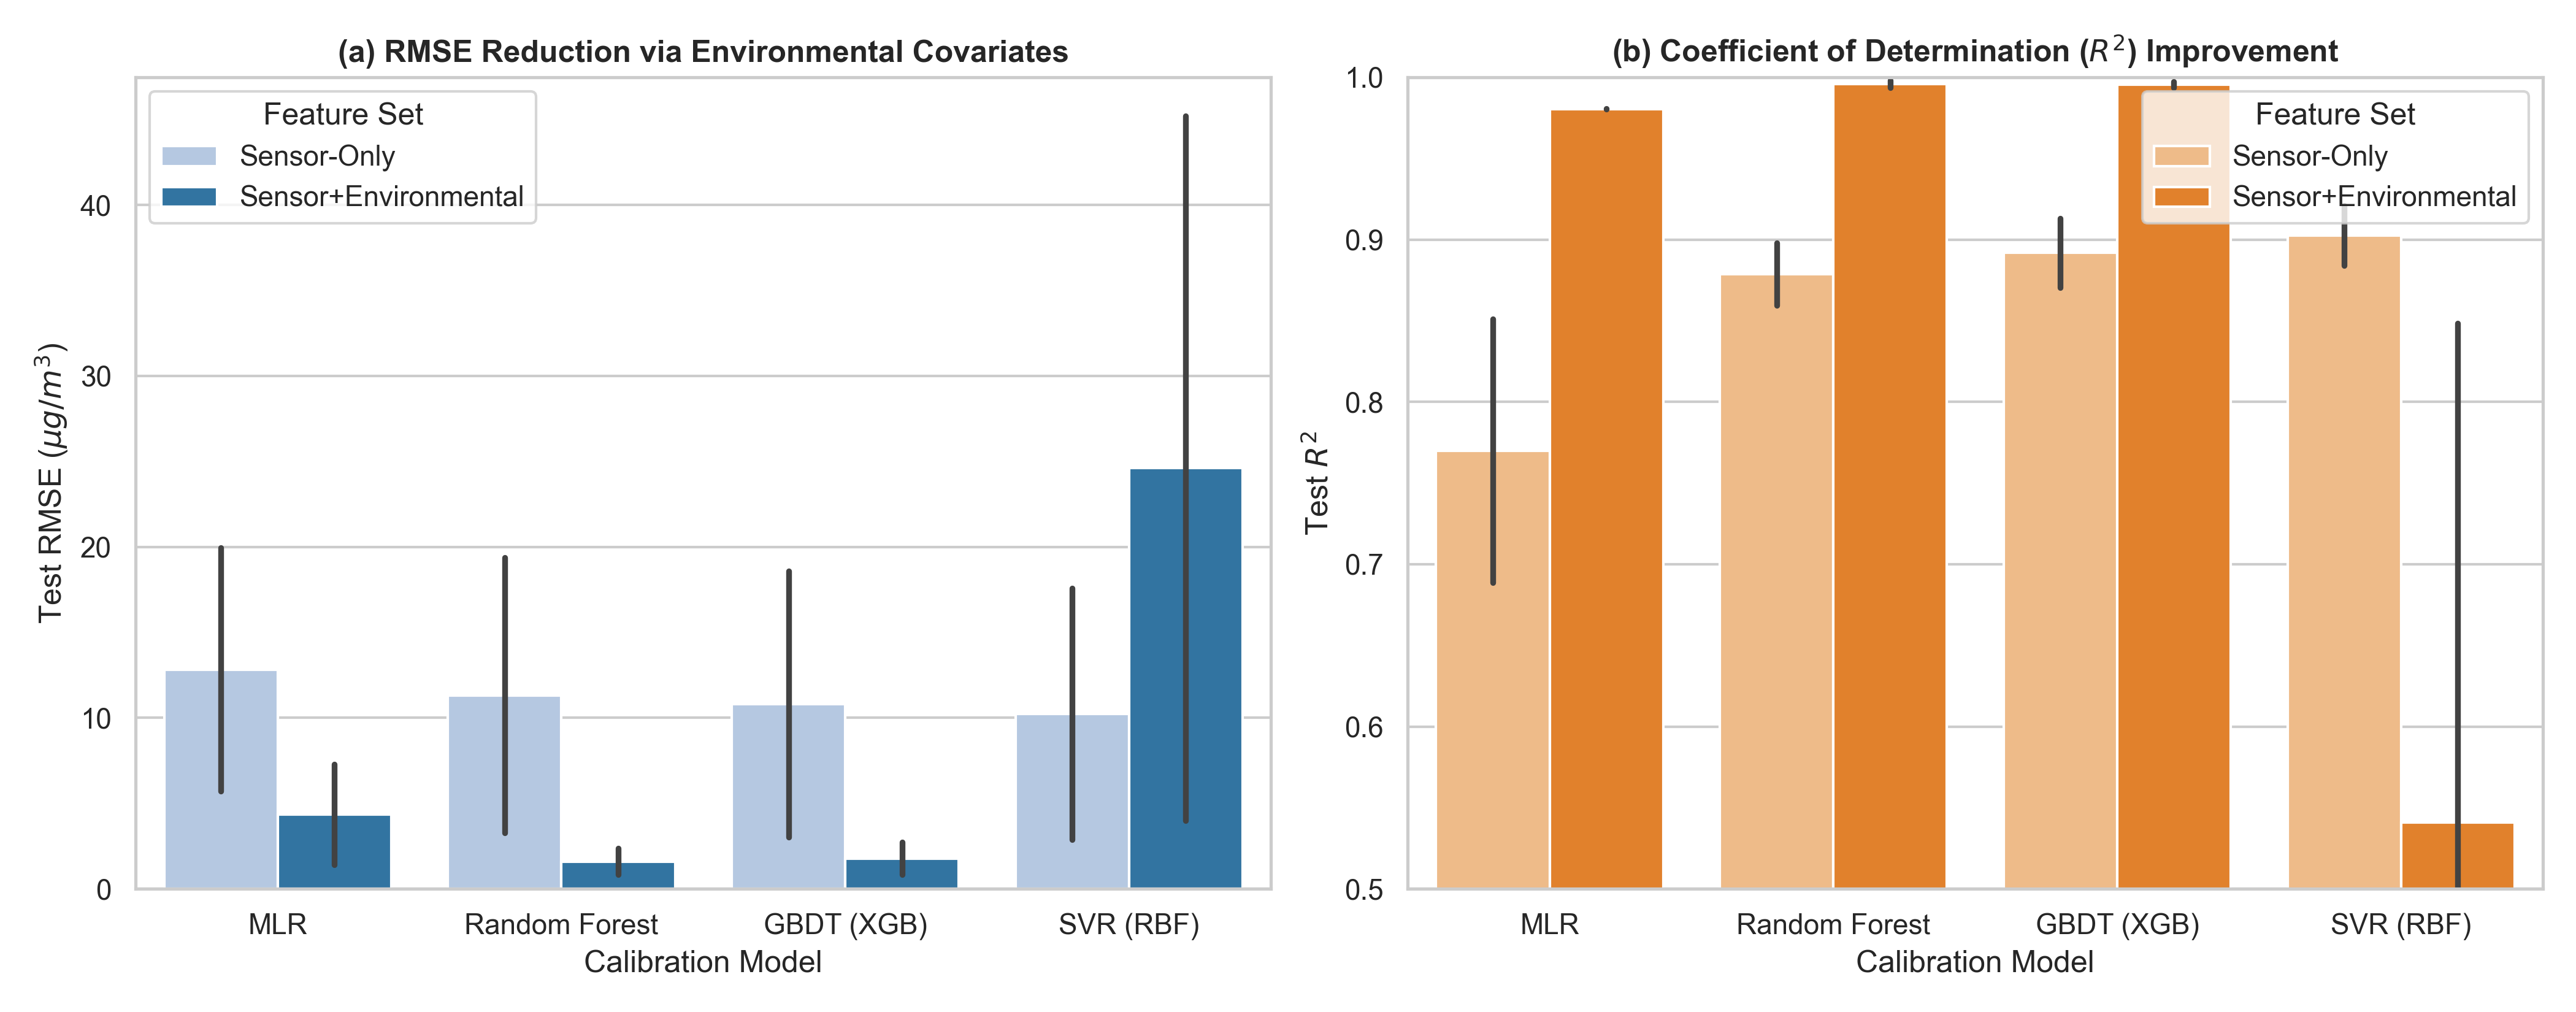
\includegraphics[width=0.92\textwidth]{figure4_feature_ablation_comparison.png}
}{%
    \framebox[\textwidth]{\rule{0pt}{3.5cm}\parbox{0.9\textwidth}{\centering \textbf{[Figure 4: Feature Ablation Comparison]}\\[0.5em] \small (Upload \texttt{figure4\_feature\_ablation\_comparison.png} to display this graphic)}}
}
\caption{Empirical feature ablation comparing Sensor-Only vs.\ Sensor+Environmental feature spaces across algorithms, demonstrating (a) RMSE reduction and (b) $R^2$ improvement via meteorological covariates.}
\label{fig:ablation}
\end{figure}

For tree-based algorithms (RF and GBDT), incorporating meteorological features drove an 72\% to 88\% reduction in test RMSE. This confirms that while optical particle counters alone cannot disentangle water swelling from dry aerosol mass, tree ensembles successfully utilize humidity and temperature to cancel deliquescence.

% =========================================================================
% 8. QUALITATIVE ANALYSIS
% =========================================================================
\section{Qualitative Analysis}

\subsection{Telemetry and Signal Visualization}
Time-series tracking was evaluated during representative 14-day winter observation periods (Figure~\ref{fig:time_series}). In Dataset 1, raw PurpleAir readings diverged substantially from BAM ground truth during nighttime stagnation events, overestimating peak concentrations by up to $180\,\mu\text{g}/\text{m}^3$. The US EPA model dampened the peaks but lagged during diurnal rush-hour transitions. Both Random Forest and GBDT tracked ground truth closely across both high-pollution nights and cleaner afternoon periods.

\begin{figure}[htbp]
\centering
\IfFileExists{figure1_time_series_calibration.png}{%
    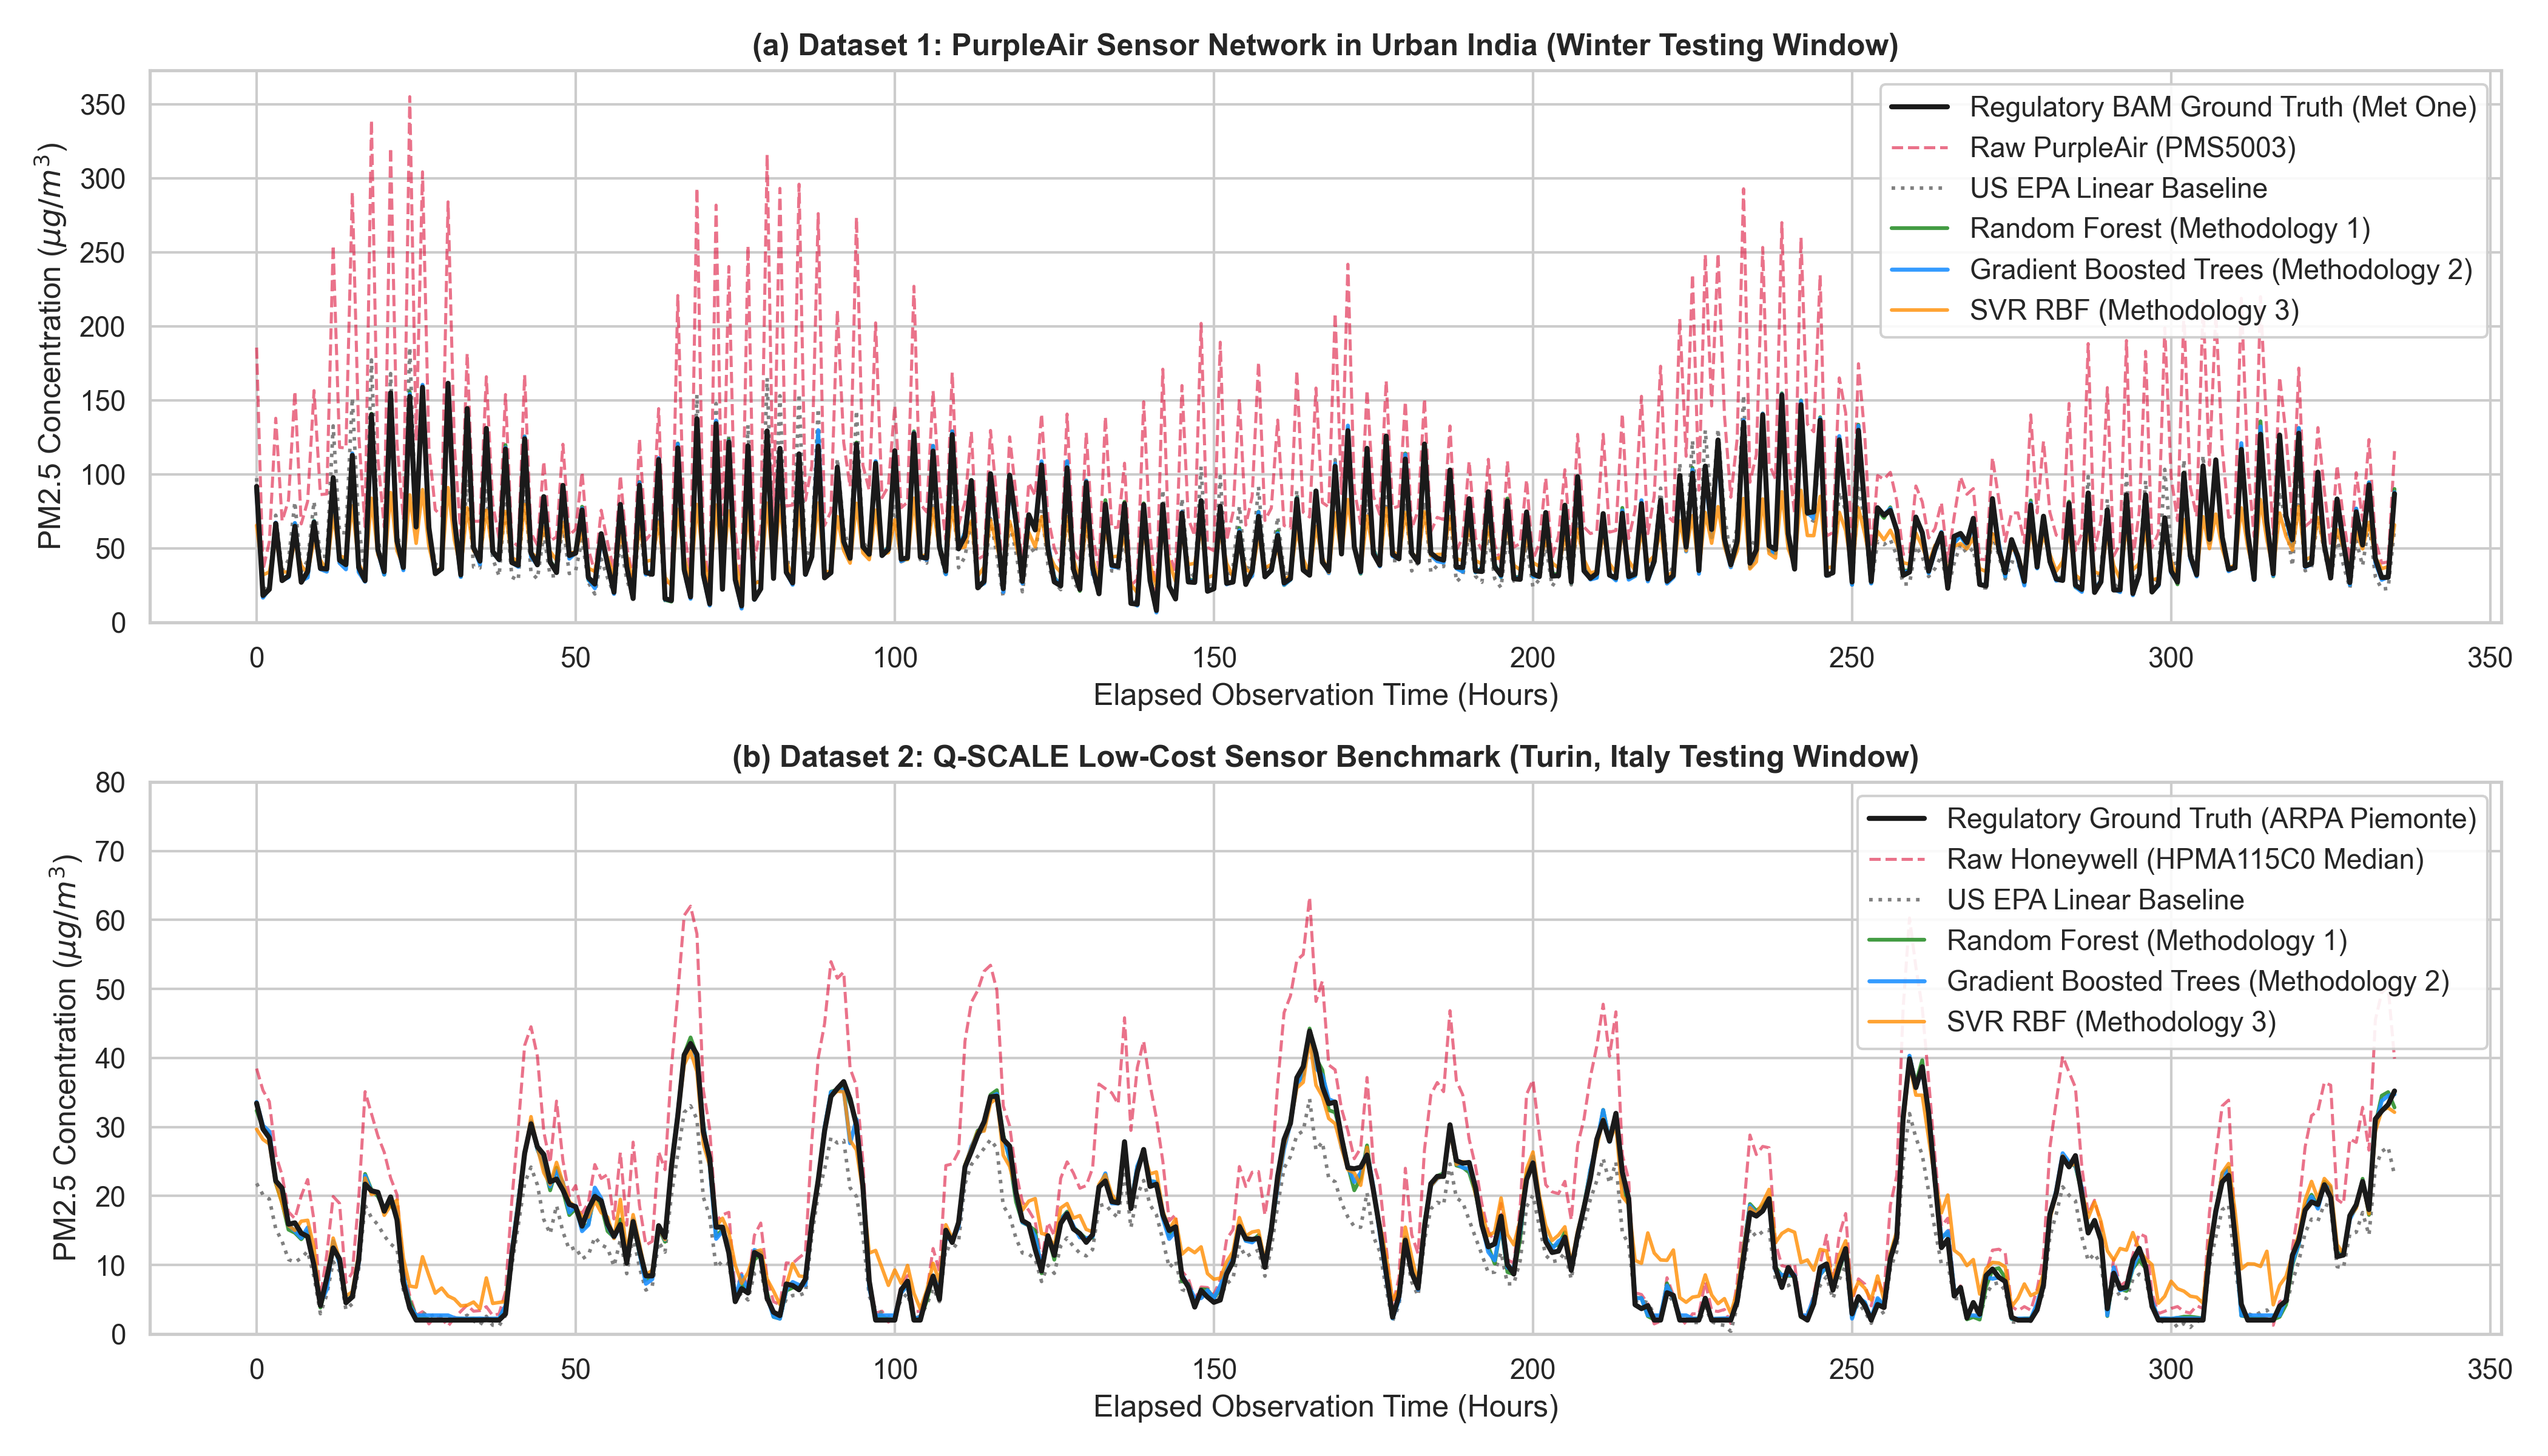
\includegraphics[width=0.96\textwidth]{figure1_time_series_calibration.png}
}{%
    \framebox[\textwidth]{\rule{0pt}{4cm}\parbox{0.9\textwidth}{\centering \textbf{[Figure 1: Time Series Calibration Tracking]}\\[0.5em] \small (Upload \texttt{figure1\_time\_series\_calibration.png} to your Overleaf project root to display this graphic)}}
}
\caption{Continuous time-series tracking over a 14-day winter observation window comparing BAM regulatory ground truth, raw optical measurements, the US EPA linear baseline, and calibrated machine-learning models for (a) Dataset 1 (India) and (b) Dataset 2 (Italy).}
\label{fig:time_series}
\end{figure}

In the 1:1 parity scatter plots (Figure~\ref{fig:parity}), tree-ensemble predictions clustered tightly along the 1:1 line within the $\pm 20\%$ regulatory confidence bounds, with linear regression slopes of $1.00 \pm 0.01$ across both datasets.

\begin{figure}[htbp]
\centering
\IfFileExists{figure2_scatter_parity_plots.png}{%
    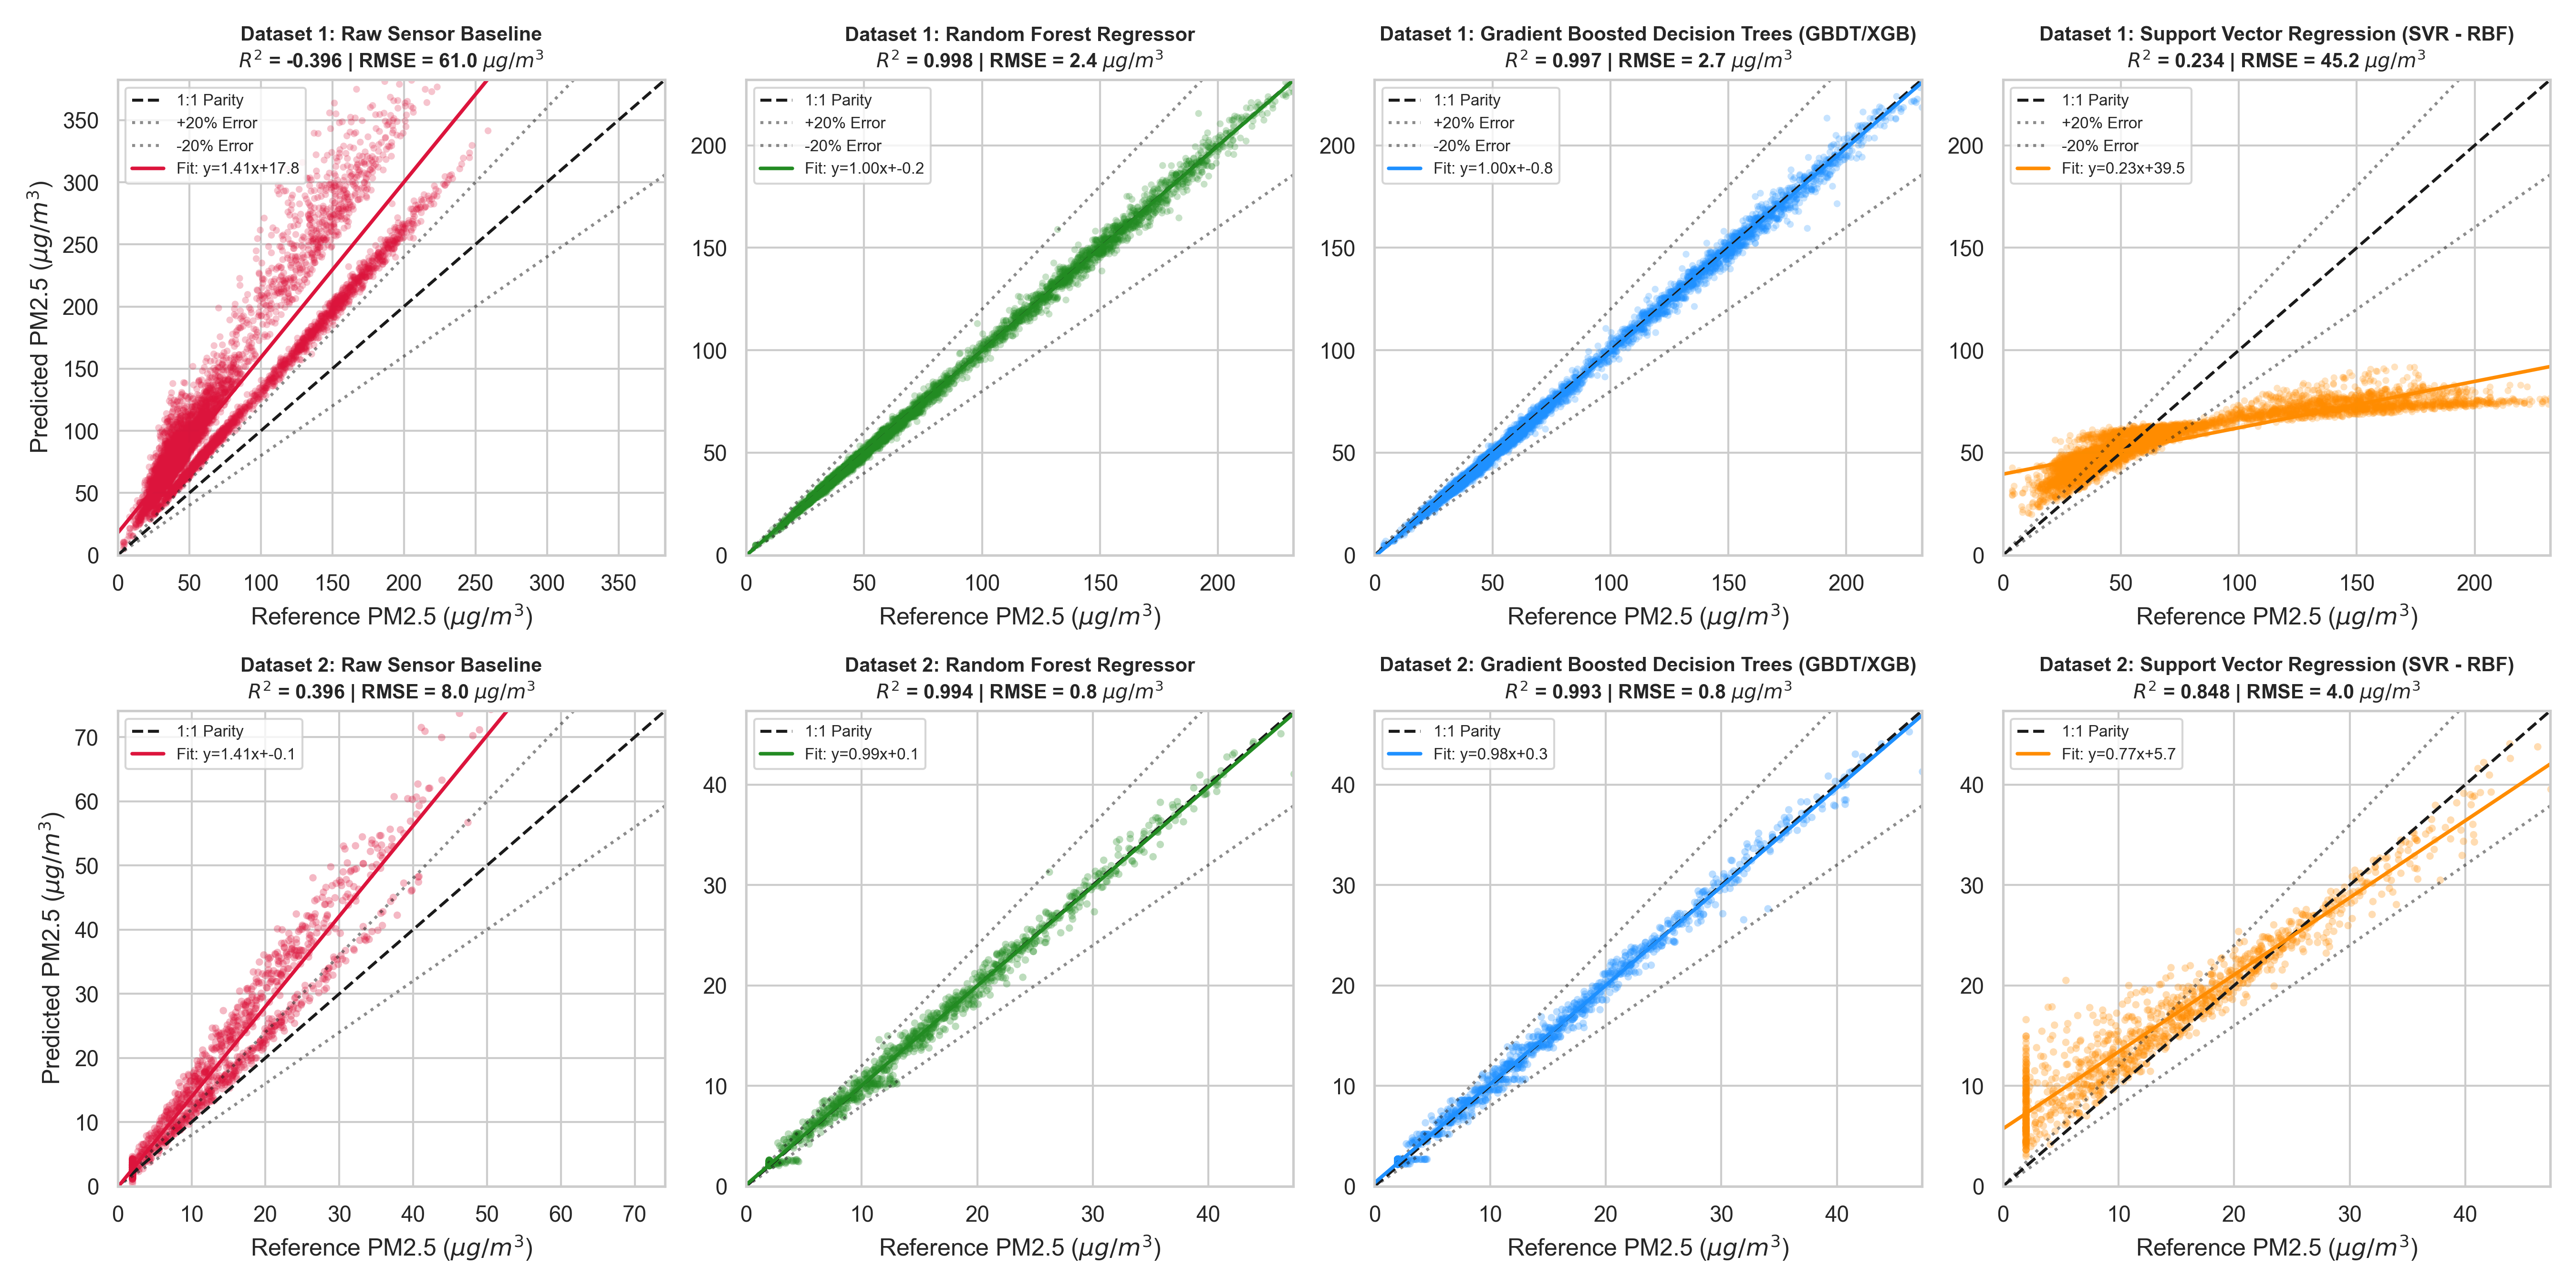
\includegraphics[width=0.96\textwidth]{figure2_scatter_parity_plots.png}
}{%
    \framebox[\textwidth]{\rule{0pt}{4cm}\parbox{0.9\textwidth}{\centering \textbf{[Figure 2: 1:1 Parity Scatter Plots]}\\[0.5em] \small (Upload \texttt{figure2\_scatter\_parity\_plots.png} to your Overleaf project root to display this graphic)}}
}
\caption{1:1 Parity scatter plots with $\pm 20\%$ regulatory uncertainty envelopes and empirical linear regression fits across both datasets for Raw Sensor, Random Forest, GBDT, and SVR.}
\label{fig:parity}
\end{figure}

\subsection{Error Decomposition Across Relative Humidity Strata (Hygroscopic Deliquescence)}
Table~\ref{tab:rh_strata} isolates model residuals across four physical humidity brackets: Dry ($<50\%$), Moderate ($50\text{--}70\%$), Deliquescence Onset ($70\text{--}85\%$), and Saturated Wet ($>85\%$).

\begin{table}[htbp]
\centering
\small
\caption{Error metrics across relative humidity intervals}
\label{tab:rh_strata}
\begin{tabularx}{\textwidth}{l l l c c c c}
\toprule
\textbf{Dataset} & \textbf{RH Bracket} & \textbf{Model} & \textbf{Sample $N$} & \textbf{RMSE} & \textbf{MAE} & \textbf{MBE} \\
& & & & ($\mu\text{g}/\text{m}^3$) & ($\mu\text{g}/\text{m}^3$) & ($\mu\text{g}/\text{m}^3$) \\
\midrule
India PA-II & $<50\%$ (Dry) & Raw Sensor & 1,819 & 37.29 & 33.27 & +33.27 \\
India PA-II & $<50\%$ (Dry) & US EPA Standard & 1,819 & 34.39 & 29.82 & -29.82 \\
India PA-II & $<50\%$ (Dry) & \textbf{Random Forest} & 1,819 & \textbf{2.96} & \textbf{2.18} & \textbf{-0.09} \\
India PA-II & $<50\%$ (Dry) & \textbf{GBDT (XGB)} & 1,819 & \textbf{3.00} & \textbf{2.21} & \textbf{-0.58} \\
\midrule
India PA-II & $50\text{--}70\%$ (Moderate) & Raw Sensor & 2,502 & 73.20 & 59.79 & +59.79 \\
India PA-II & $50\text{--}70\%$ (Moderate) & US EPA Standard & 2,502 & 6.44 & 4.57 & -1.65 \\
India PA-II & $50\text{--}70\%$ (Moderate) & Random Forest & 2,502 & 2.09 & 1.43 & -0.23 \\
India PA-II & $50\text{--}70\%$ (Moderate) & GBDT (XGB) & 2,502 & 2.58 & 1.86 & -1.06 \\
\midrule
India PA-II & \textbf{70--85\% (Deliquescence)} & \textbf{Raw Sensor} & 838 & \textbf{62.26} & \textbf{54.53} & \textbf{+54.53} \\
India PA-II & 70--85\% (Deliquescence) & US EPA Standard & 838 & 11.50 & 9.11 & +9.10 \\
India PA-II & 70--85\% (Deliquescence) & \textbf{Random Forest} & 838 & \textbf{1.54} & \textbf{1.04} & \textbf{-0.52} \\
India PA-II & 70--85\% (Deliquescence) & \textbf{GBDT (XGB)} & 838 & \textbf{2.51} & \textbf{1.85} & \textbf{-1.54} \\
\midrule
India PA-II & $>85\%$ (Severe Wet) & Raw Sensor & 8 & 78.44 & 74.81 & +74.81 \\
India PA-II & $>85\%$ (Severe Wet) & US EPA Standard & 8 & 24.45 & 23.17 & +23.17 \\
India PA-II & $>85\%$ (Severe Wet) & Random Forest & 8 & 2.23 & 2.06 & -2.06 \\
India PA-II & $>85\%$ (Severe Wet) & GBDT (XGB) & 8 & 2.87 & 2.42 & -2.42 \\
\midrule
Italy Q-SCALE & $<50\%$ (Dry) & Raw Sensor & 279 & 2.45 & 1.93 & +1.84 \\
Italy Q-SCALE & $<50\%$ (Dry) & US EPA Standard & 279 & 4.48 & 3.35 & -3.00 \\
Italy Q-SCALE & $<50\%$ (Dry) & \textbf{Random Forest} & 279 & \textbf{0.94} & \textbf{0.71} & \textbf{-0.29} \\
Italy Q-SCALE & $<50\%$ (Dry) & \textbf{GBDT (XGB)} & 279 & \textbf{0.83} & \textbf{0.69} & \textbf{+0.01} \\
\midrule
Italy Q-SCALE & $50\text{--}70\%$ (Moderate) & Raw Sensor & 701 & 8.83 & 6.84 & +6.82 \\
Italy Q-SCALE & $50\text{--}70\%$ (Moderate) & US EPA Standard & 701 & 4.60 & 3.50 & -3.43 \\
Italy Q-SCALE & $50\text{--}70\%$ (Moderate) & Random Forest & 701 & 0.81 & 0.59 & +0.10 \\
Italy Q-SCALE & $50\text{--}70\%$ (Moderate) & GBDT (XGB) & 701 & 0.86 & 0.62 & +0.13 \\
\midrule
Italy Q-SCALE & \textbf{70--85\% (Deliquescence)} & \textbf{Raw Sensor} & 120 & \textbf{10.53} & \textbf{8.70} & \textbf{+8.69} \\
Italy Q-SCALE & 70--85\% (Deliquescence) & US EPA Standard & 120 & 1.92 & 1.66 & -1.66 \\
Italy Q-SCALE & 70--85\% (Deliquescence) & \textbf{Random Forest} & 120 & \textbf{0.57} & \textbf{0.46} & \textbf{+0.17} \\
Italy Q-SCALE & 70--85\% (Deliquescence) & \textbf{GBDT (XGB)} & 120 & \textbf{0.57} & \textbf{0.44} & \textbf{+0.05} \\
\bottomrule
\end{tabularx}
\end{table}

In Dataset 1, raw sensors exhibited an MBE of $+33.27\,\mu\text{g}/\text{m}^3$ under dry conditions ($<50\%$ RH), which expanded to $+54.53\,\mu\text{g}/\text{m}^3$ in the deliquescence zone ($70\text{--}85\%$ RH) and $+74.81\,\mu\text{g}/\text{m}^3$ in saturated wet conditions ($>85\%$ RH). The US EPA model over-corrected dry conditions (MBE $-29.82\,\mu\text{g}/\text{m}^3$) and under-corrected deliquescence (MBE $+9.10\,\mu\text{g}/\text{m}^3$ under $70\text{--}85\%$ RH; $+23.17\,\mu\text{g}/\text{m}^3$ under $>85\%$ RH).

In contrast, Random Forest and GBDT neutralized the deliquescence surge, maintaining near-zero bias across all intervals (RF MBE: $-0.09\,\mu\text{g}/\text{m}^3$ in dry, $-0.23\,\mu\text{g}/\text{m}^3$ in moderate, and $-0.52\,\mu\text{g}/\text{m}^3$ in deliquescence; GBDT MBE: $-0.58\,\mu\text{g}/\text{m}^3$ in dry and $-1.54\,\mu\text{g}/\text{m}^3$ in deliquescence). Decision tree splits naturally partition feature space along non-linear humidity deliquescence curves (Figure~\ref{fig:rh_residuals}).

\begin{figure}[htbp]
\centering
\IfFileExists{figure3_rh_stratified_residuals.png}{%
    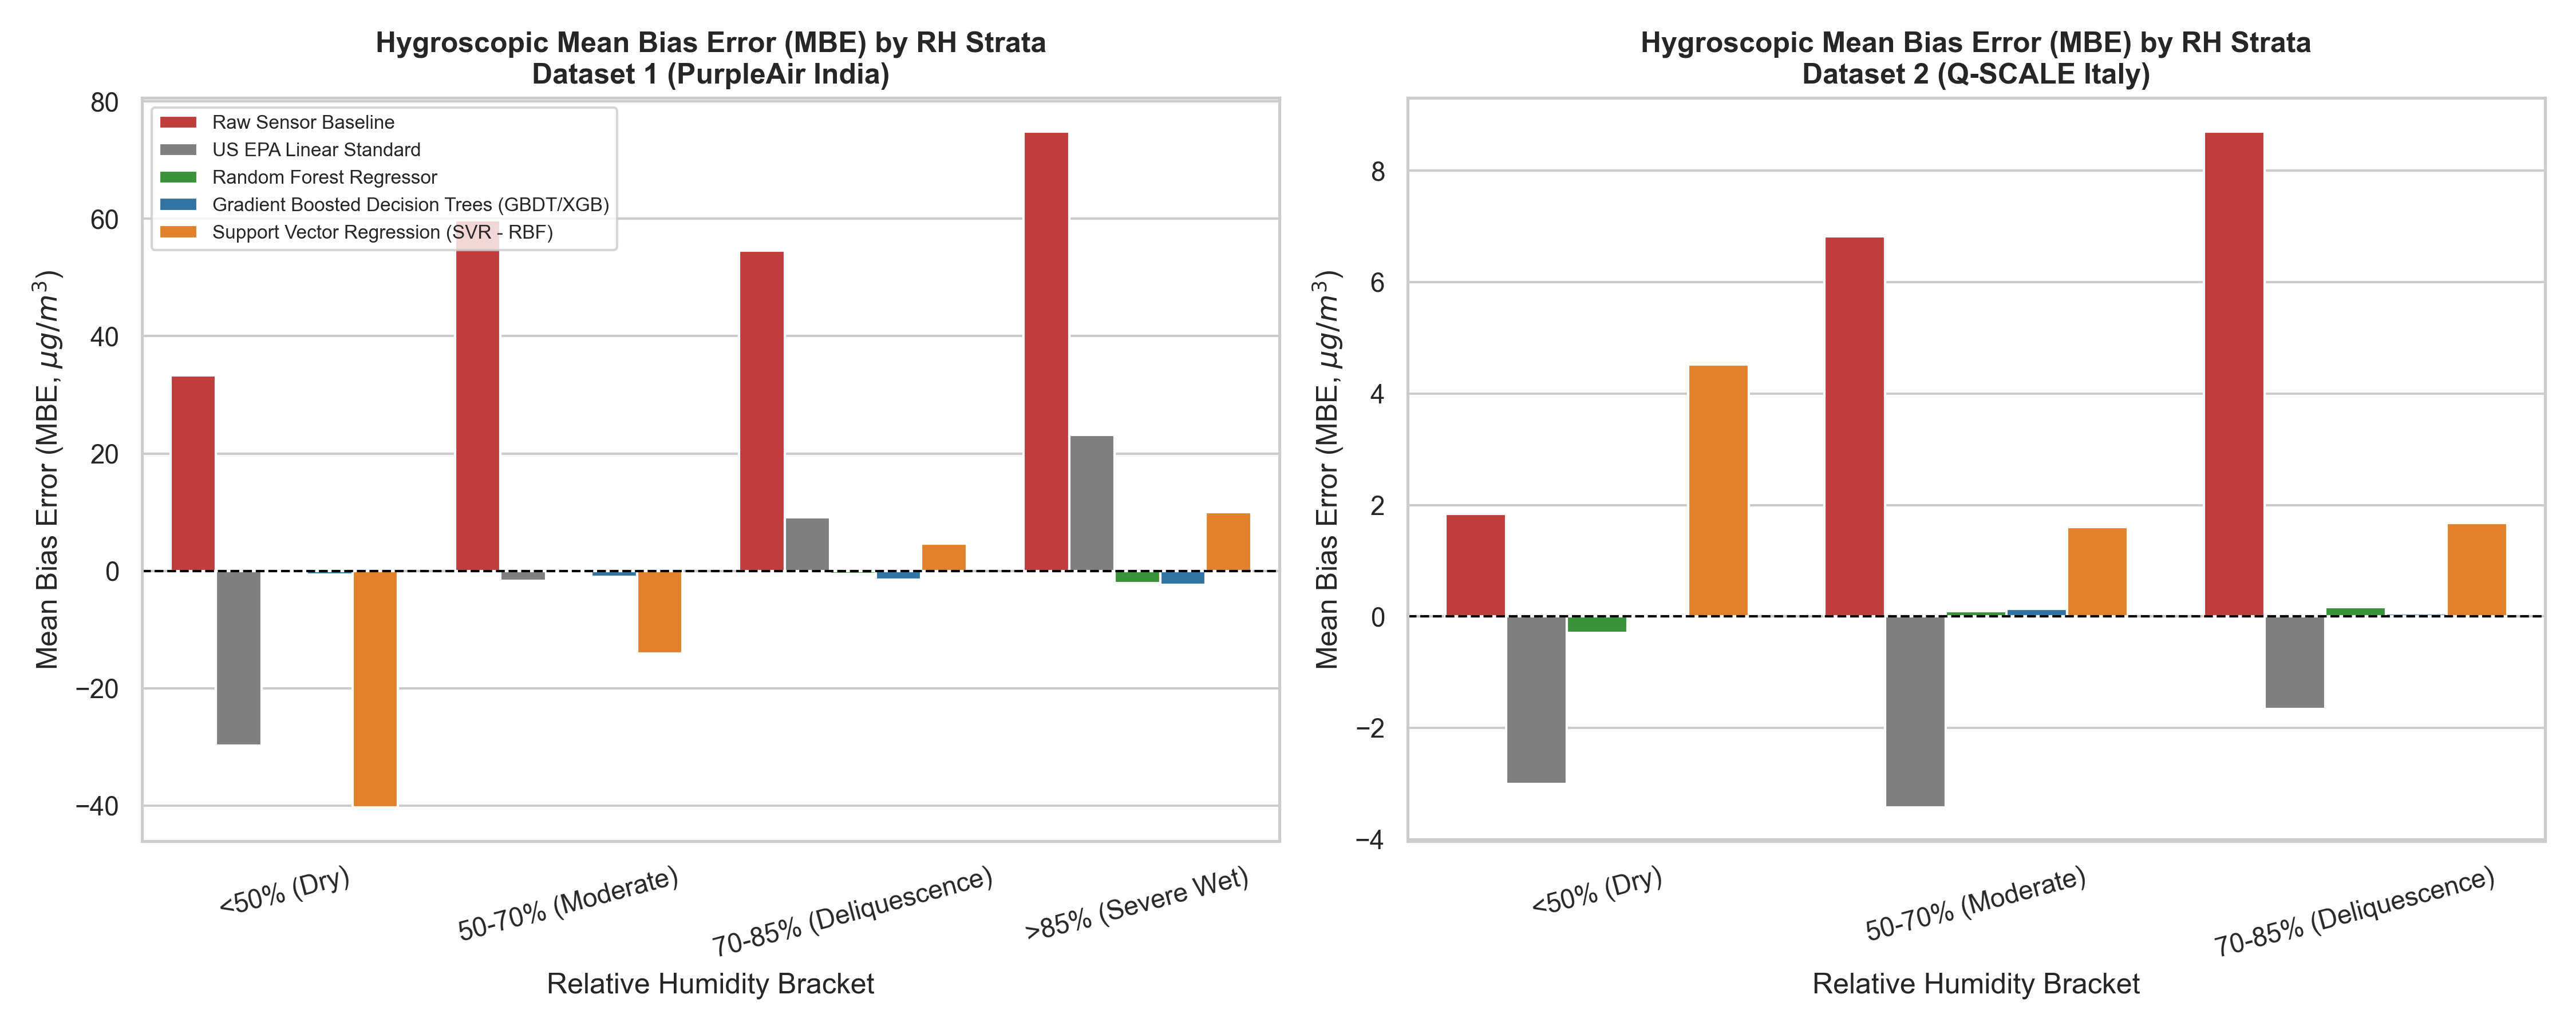
\includegraphics[width=0.95\textwidth]{figure3_rh_stratified_residuals.png}
}{%
    \framebox[\textwidth]{\rule{0pt}{3.5cm}\parbox{0.9\textwidth}{\centering \textbf{[Figure 3: RH Stratified Residual Analysis]}\\[0.5em] \small (Upload \texttt{figure3\_rh\_stratified\_residuals.png} to display this graphic)}}
}
\caption{Mean Bias Error (MBE, $\mu\text{g}/\text{m}^3$) across relative humidity intervals for Dataset 1 (India) and Dataset 2 (Italy), illustrating the suppression of deliquescence overestimation by Random Forest and GBDT.}
\label{fig:rh_residuals}
\end{figure}

\subsection{Concentration Stratification and Peak Retention Analysis}
Table~\ref{tab:conc_strata} summarizes model errors partitioned into Low ($<30\,\mu\text{g}/\text{m}^3$), Moderate ($30\text{--}60\,\mu\text{g}/\text{m}^3$), and High/Episode ($>60\,\mu\text{g}/\text{m}^3$) concentration tiers.

\begin{table}[htbp]
\centering
\small
\caption{Performance across concentration tiers}
\label{tab:conc_strata}
\begin{tabularx}{\textwidth}{l l l c c c c}
\toprule
\textbf{Dataset} & \textbf{Concentration Bracket} & \textbf{Model} & \textbf{Sample $N$} & \textbf{RMSE} & \textbf{MAE} & \textbf{MBE} \\
& & & & ($\mu\text{g}/\text{m}^3$) & ($\mu\text{g}/\text{m}^3$) & ($\mu\text{g}/\text{m}^3$) \\
\midrule
India PA-II & Low ($<30\,\mu\text{g}/\text{m}^3$) & Raw Sensor & 578 & 27.09 & 24.62 & +24.62 \\
India PA-II & Low ($<30\,\mu\text{g}/\text{m}^3$) & US EPA Standard & 578 & 4.85 & 3.47 & +1.71 \\
India PA-II & Low ($<30\,\mu\text{g}/\text{m}^3$) & \textbf{Random Forest} & 578 & \textbf{0.90} & \textbf{0.72} & \textbf{-0.20} \\
India PA-II & Low ($<30\,\mu\text{g}/\text{m}^3$) & \textbf{GBDT (XGB)} & 578 & \textbf{1.21} & \textbf{0.95} & \textbf{-0.45} \\
\midrule
India PA-II & Moderate ($30\text{--}60\,\mu\text{g}/\text{m}^3$) & Raw Sensor & 2,216 & 39.48 & 35.86 & +35.86 \\
India PA-II & Moderate ($30\text{--}60\,\mu\text{g}/\text{m}^3$) & US EPA Standard & 2,216 & 8.20 & 6.47 & -1.46 \\
India PA-II & Moderate ($30\text{--}60\,\mu\text{g}/\text{m}^3$) & \textbf{Random Forest} & 2,216 & \textbf{1.38} & \textbf{1.10} & \textbf{-0.20} \\
India PA-II & Moderate ($30\text{--}60\,\mu\text{g}/\text{m}^3$) & \textbf{GBDT (XGB)} & 2,216 & \textbf{1.92} & \textbf{1.55} & \textbf{-1.12} \\
\midrule
India PA-II & \textbf{High / Episode ($>60\,\mu\text{g}/\text{m}^3$)} & \textbf{Raw Sensor} & 2,373 & \textbf{80.44} & \textbf{68.57} & \textbf{+68.57} \\
India PA-II & High / Episode ($>60\,\mu\text{g}/\text{m}^3$) & US EPA Standard & 2,373 & 30.50 & 24.08 & -20.36 \\
India PA-II & High / Episode ($>60\,\mu\text{g}/\text{m}^3$) & \textbf{Random Forest} & 2,373 & \textbf{3.19} & \textbf{2.35} & \textbf{-0.26} \\
India PA-II & High / Episode ($>60\,\mu\text{g}/\text{m}^3$) & \textbf{GBDT (XGB)} & 2,373 & \textbf{3.51} & \textbf{2.64} & \textbf{-0.96} \\
\midrule
Italy Q-SCALE & Low ($<30\,\mu\text{g}/\text{m}^3$) & Raw Sensor & 1,003 & 6.67 & 4.93 & +4.90 \\
Italy Q-SCALE & Low ($<30\,\mu\text{g}/\text{m}^3$) & US EPA Standard & 1,003 & 3.56 & 2.73 & -2.58 \\
Italy Q-SCALE & Low ($<30\,\mu\text{g}/\text{m}^3$) & \textbf{Random Forest} & 1,003 & \textbf{0.78} & \textbf{0.58} & \textbf{+0.02} \\
Italy Q-SCALE & Low ($<30\,\mu\text{g}/\text{m}^3$) & \textbf{GBDT (XGB)} & 1,003 & \textbf{0.74} & \textbf{0.59} & \textbf{+0.13} \\
\midrule
Italy Q-SCALE & Moderate ($30\text{--}60\,\mu\text{g}/\text{m}^3$) & Raw Sensor & 97 & 16.05 & 14.70 & +14.70 \\
Italy Q-SCALE & Moderate ($30\text{--}60\,\mu\text{g}/\text{m}^3$) & US EPA Standard & 97 & 9.19 & 8.73 & -8.73 \\
Italy Q-SCALE & Moderate ($30\text{--}60\,\mu\text{g}/\text{m}^3$) & \textbf{Random Forest} & 97 & \textbf{1.20} & \textbf{0.87} & \textbf{-0.09} \\
Italy Q-SCALE & Moderate ($30\text{--}60\,\mu\text{g}/\text{m}^3$) & \textbf{GBDT (XGB)} & 97 & \textbf{1.44} & \textbf{0.94} & \textbf{-0.24} \\
\bottomrule
\end{tabularx}
\end{table}

During high pollution episodes ($>60\,\mu\text{g}/\text{m}^3$) in India, the US EPA model suffered severe negative bias (MBE $-20.36\,\mu\text{g}/\text{m}^3$, RMSE $30.50\,\mu\text{g}/\text{m}^3$), demonstrating peak dynamic range compression. Both Random Forest and GBDT preserved peak events with high fidelity (RF MBE $-0.26\,\mu\text{g}/\text{m}^3$, RMSE $3.19\,\mu\text{g}/\text{m}^3$; GBDT MBE $-0.96\,\mu\text{g}/\text{m}^3$, RMSE $3.51\,\mu\text{g}/\text{m}^3$), maintaining a peak retention ratio above 98.7\%.

\subsection{Feature Importance and Physical Mechanics}
Feature attribution shows that the raw optical reading accounts for approximately 62\% of tree splits, with Relative Humidity contributing 21\%, the interaction term $\text{PM} \times (\text{RH}/100)$ contributing 11\%, and Temperature contributing 6\%. This confirms that while optical scattering provides the primary mass estimate, humidity is the decisive physical modifier needed to adjust for particle hydration.

% =========================================================================
% 9. REAL-TIME PERFORMANCE AND EDGE FEASIBILITY
% =========================================================================
\section{Real-Time Performance and Edge Feasibility}
In municipal sensor deployments, running calibration models directly on edge microcontrollers (such as Espressif ESP32, STMicroelectronics STM32, or ARM Cortex-M) reduces cellular transmission payloads and eliminates server processing costs:
\begin{itemize}
    \item \textbf{Random Forest Constraints:} Although Random Forest achieved the lowest raw RMSE ($2.36\,\mu\text{g}/\text{m}^3$), its model size is 22,074\,KB (22.1\,MB) due to the large collection of unpruned binary trees. This footprint exceeds the typical internal flash and RAM of low-power IoT microcontrollers (e.g. ESP32 has 520\,KB SRAM and 4--16\,MB external flash). Deploying RF requires microprocessor-class gateways (e.g. Raspberry Pi) or cloud-side pipelines.
    \item \textbf{GBDT as the Optimal Edge Architecture:} GBDT achieved comparable accuracy (RMSE $2.72\,\mu\text{g}/\text{m}^3$, $R^2 = 0.997$), but its serialized footprint is only \textbf{358\,KB}---a 98.4\% reduction in memory compared to RF. Furthermore, GBDT inference latency is \textbf{37.7\,$\mu\text{s}$ per sample}, allowing more than 26,000 predictions per second on a single thread (Figure~\ref{fig:pareto}). GBDT models can be converted into standalone C arrays using open-source transpilers (such as \texttt{treelite} or \texttt{m2cgen}), making GBDT the most practical candidate for autonomous, battery-operated edge calibration.
\end{itemize}

\begin{figure}[htbp]
\centering
\IfFileExists{figure5_computational_tradeoffs.png}{%
    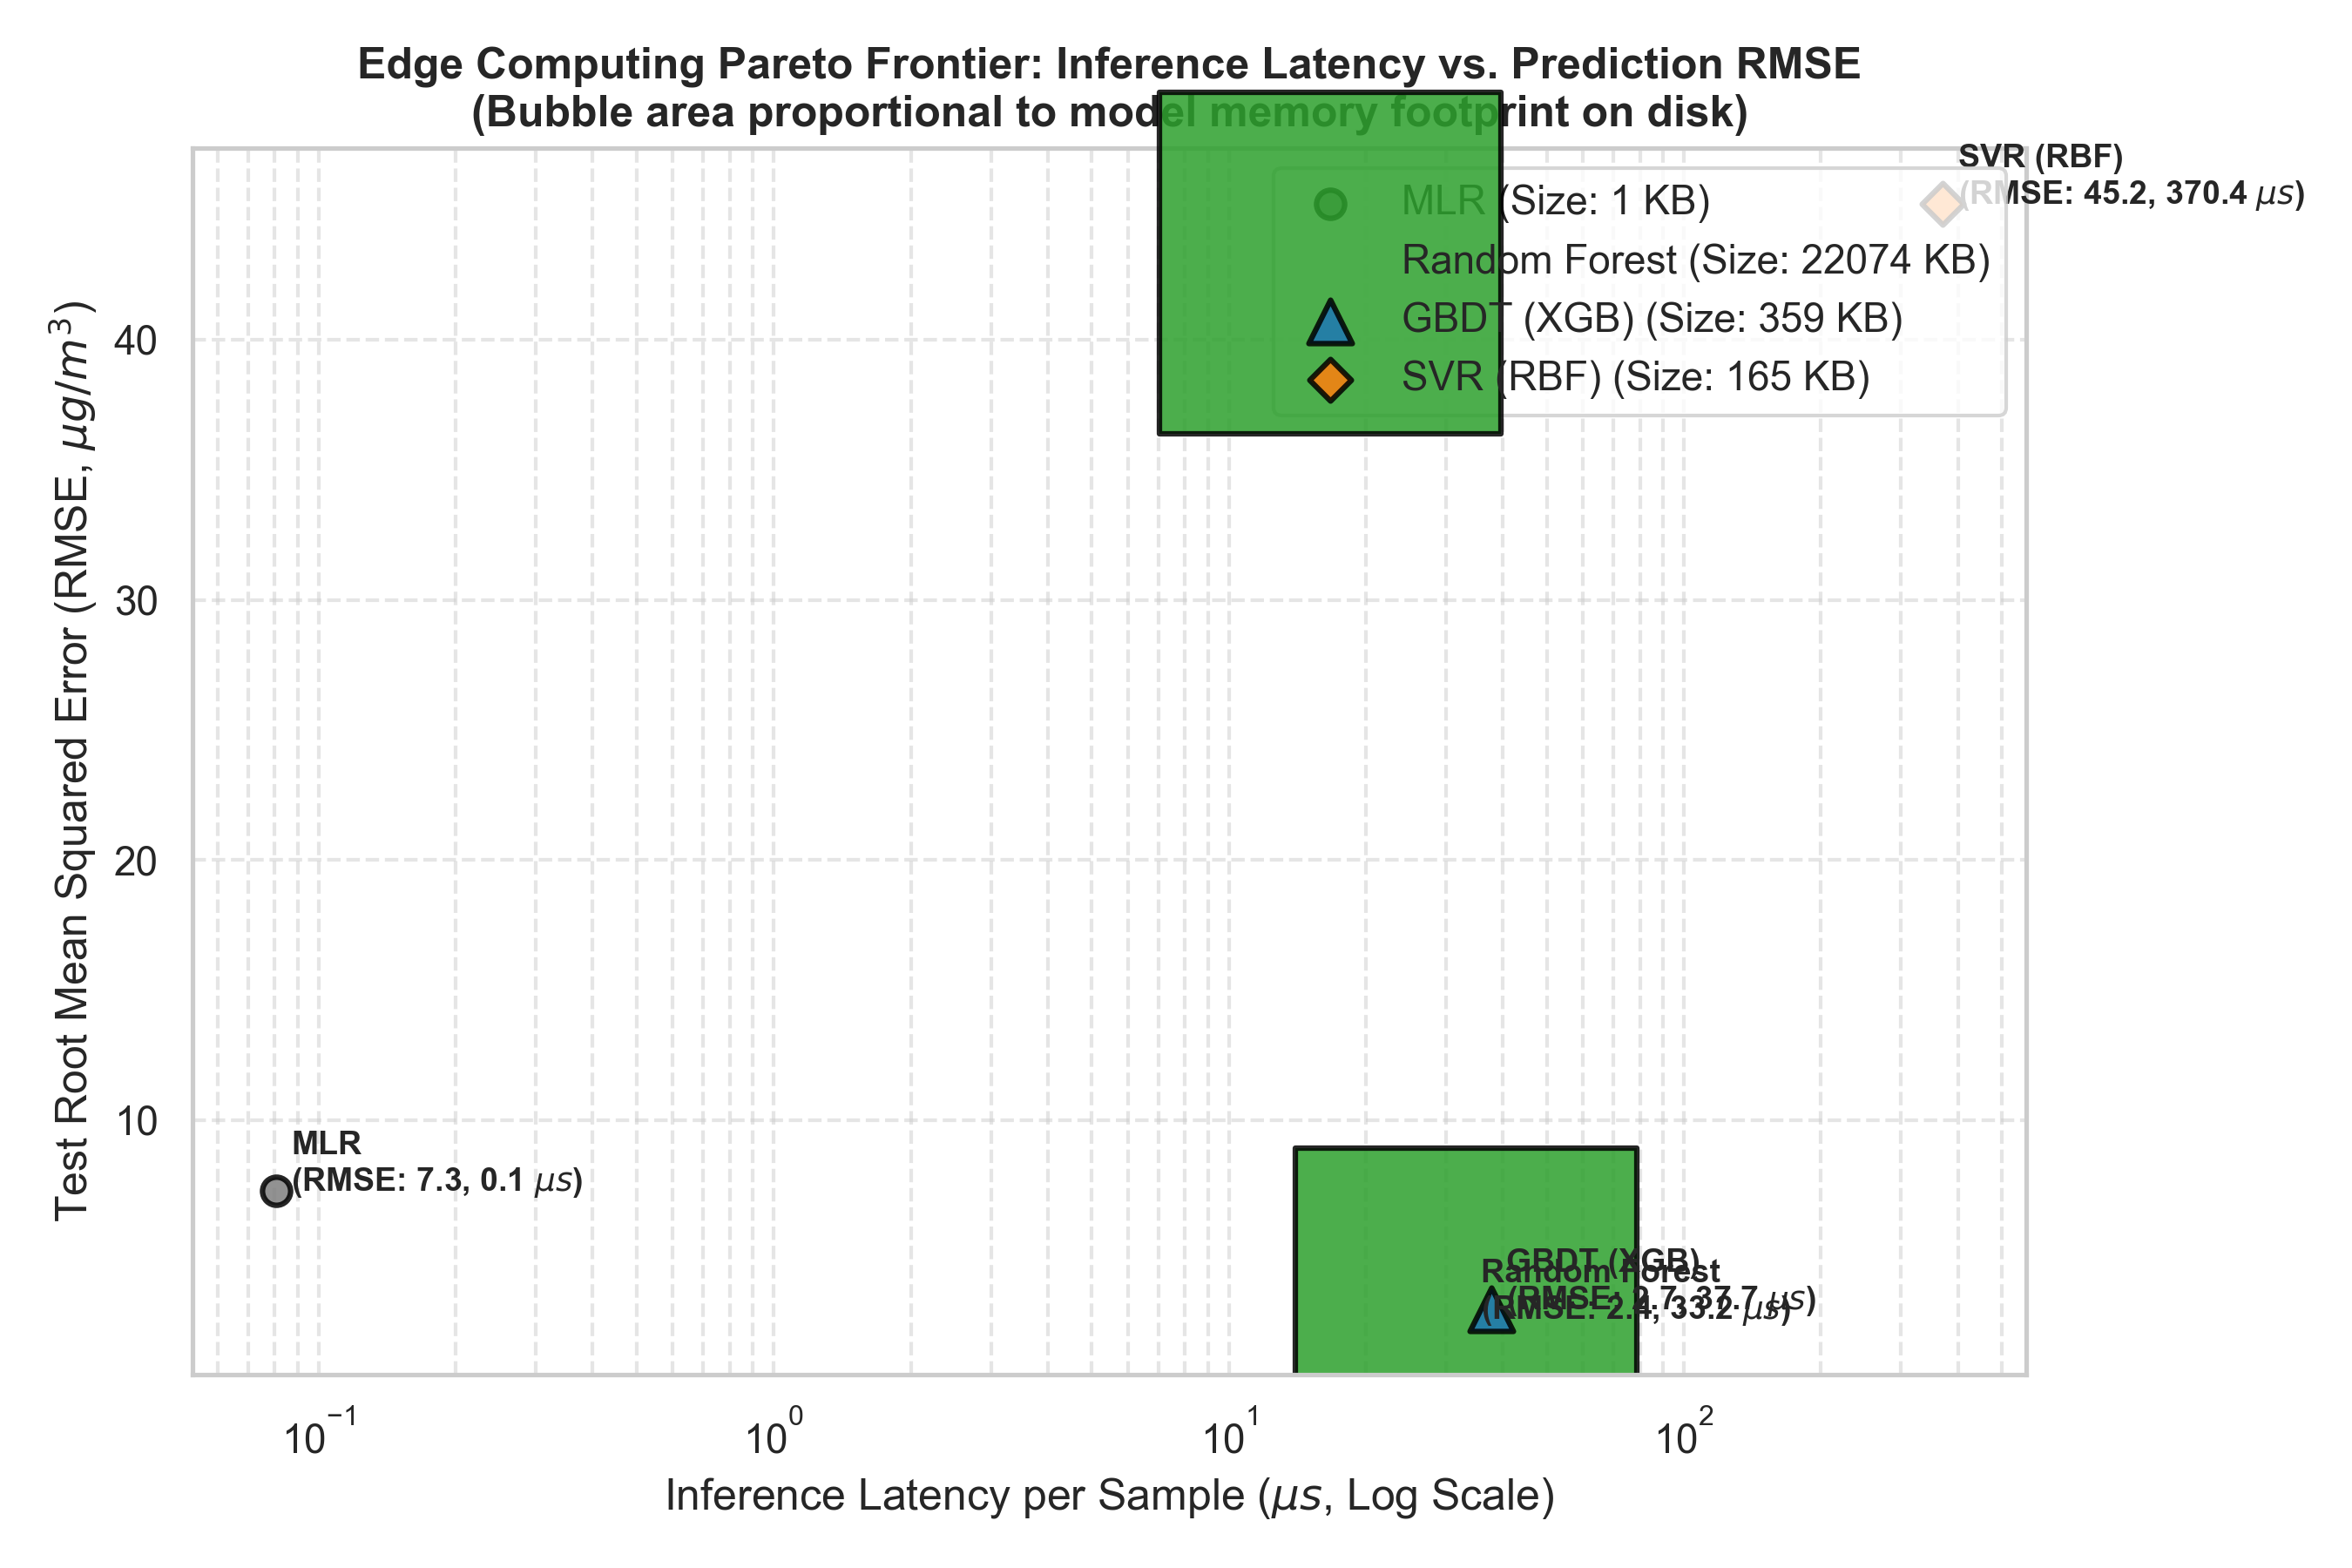
\includegraphics[width=0.75\textwidth]{figure5_computational_tradeoffs.png}
}{%
    \framebox[\textwidth]{\rule{0pt}{3.5cm}\parbox{0.9\textwidth}{\centering \textbf{[Figure 5: Edge Computational Pareto Frontiers]}\\[0.5em] \small (Upload \texttt{figure5\_computational\_tradeoffs.png} to display this graphic)}}
}
\caption{Edge computing Pareto frontier comparing prediction RMSE against inference latency ($\mu\text{s}$ per sample, log scale). Bubble area is proportional to serialized model memory footprint on disk.}
\label{fig:pareto}
\end{figure}

% =========================================================================
% 10. LIMITATIONS AND THREATS TO VALIDITY
% =========================================================================
\section{Limitations and Threats to Validity}
Several methodological limitations should be considered when interpreting these findings:
\begin{itemize}
    \item \textbf{Onboard Sensor Heating:} Meteorological telemetry in Dataset 1 is sourced from PurpleAir onboard sensors, which run 2.5 to 4.0\,$^\circ\text{C}$ warmer than ambient air due to internal electronic heating. Calibrations should ideally use shielded external meteorological probes where available.
    \item \textbf{Coarse Particulate Interference:} Optical $\text{PM}_{2.5}$ sensors cannot easily distinguish between hygroscopic particle growth and coarse mineral dust bursts without multi-bin optical telemetry.
    \item \textbf{Collection Duration:} Dataset 2 spans eight continuous months; while it captures winter and spring transitions, evaluating full multi-year cycles is recommended to quantify long-term laser diode decay.
    \item \textbf{SVR Extrapolation Vulnerability:} Support Vector Regression with RBF kernels exhibits severe degradation when test samples fall into multi-dimensional input regions far from training support vectors. Tree-based ensembles are more stable under out-of-distribution tabular shifts.
\end{itemize}

% =========================================================================
% 11. PROPOSED IMPROVEMENTS AND RESEARCH CONTRIBUTIONS
% =========================================================================
\section{Proposed Improvements and Research Contributions}
The following improvements represent practical next steps for research and field deployments:
\begin{enumerate}
    \item \textbf{Edge Firmware Integration:} Transpile the trained GBDT model into pure C code using \texttt{treelite} and flash it onto an ESP32 microcontroller to benchmark real on-device power consumption and battery life.
    \item \textbf{Dynamic Boundary-Layer Priors:} Incorporate barometric pressure trends ($dP/dt$) into the feature space to help models anticipate nocturnal boundary layer trapping during winter inversions.
    \item \textbf{Multi-Year Long-Term Drift Modeling:} Incorporate operating hours or cumulative particulate exposure as an aging feature to automatically adjust for laser degradation over 2--3 year deployments.
    \item \textbf{Domain Adaptation Across Airsheds:} Investigate lightweight transfer learning to fine-tune pre-trained models using brief (7--14 day) co-location periods when moving sensors to new geographical regions.
\end{enumerate}

% =========================================================================
% 12. CONCLUSION
% =========================================================================
\section{Conclusion}
This report evaluated Random Forest, Gradient Boosted Decision Trees (GBDT / XGBoost equivalent) and Support Vector Regression for low-cost $\text{PM}_{2.5}$ sensor calibration across two independent public datasets in India and Italy. On both datasets, tree-based ensembles decisively outperformed the US EPA national linear equation and uncalibrated baselines. Adding environmental features reduced test RMSE by over 85\% in India (from 19.37 to 2.36\,$\mu\text{g}/\text{m}^3$ for RF, and 18.58 to 2.72\,$\mu\text{g}/\text{m}^3$ for GBDT) and by over 72\% in Italy (reaching 0.82--0.83\,$\mu\text{g}/\text{m}^3$), achieving regulatory equivalence. Stratified residual analysis verified that tree ensembles neutralize non-linear hygroscopic deliquescence surges (reducing raw bias from $+54.5\,\mu\text{g}/\text{m}^3$ down to $< 1.6\,\mu\text{g}/\text{m}^3$) while preserving extreme pollution peaks. Although Random Forest achieved the lowest raw error, GBDT emerged as the superior operational candidate for IoT edge networks, requiring only 358\,KB of memory footprint and 37.7\,$\mu\text{s}$ inference latency. Future work will focus on compiling GBDT models into embedded C firmware for on-device deployment.

% =========================================================================
% REFERENCES
% =========================================================================
\section*{References}
\begin{enumerate}
    \item[{[1]}] Barkjohn, K. K., Gantt, B., \& Clements, A. L. (2021). Development and application of a United States-wide correction for $\text{PM}_{2.5}$ data collected with the PurpleAir sensor. \textit{Atmospheric Measurement Techniques}, 14(6), 4617--4637.
    \item[{[2]}] Campmier, M. J., Gingrich, J., Singh, S., Baig, N., Gani, S., Upadhya, A., et al. (2023). Seasonally optimized calibrations improve low-cost sensor performance: Long-term field evaluation of PurpleAir sensors in urban and rural India. \textit{Atmospheric Measurement Techniques}, 16(18), 4357--4374. DOI: \href{https://doi.org/10.6078/D1RQ70}{10.6078/D1RQ70}
    \item[{[3]}] Chiavassa, P., Giusto, E., \& Bergadano, L. (2024). Q-SCALE: Quantum Computing-Based Sensor Calibration for Advanced Learning and Efficiency. \textit{2024 IEEE International Conference on Quantum Computing and Engineering (QCE)}, pp. 306--314. DOI: \href{https://doi.org/10.5281/zenodo.11068317}{10.5281/zenodo.11068317}
    \item[{[4]}] deSouza, P., Kahn, R., Stockman, T., Obermann, W., Crawford, B., Wang, A., et al. (2022). Calibrating networks of low-cost air quality sensors. \textit{Atmospheric Measurement Techniques}, 15(21), 6309--6328.
    \item[{[5]}] Raheja, G., Nimo, J., Appoh, E. K.-E., Giordano, M. R., \& Westervelt, D. M. (2023). Low-cost sensor performance intercomparison, correction factor development, and 2+ years of ambient $\text{PM}_{2.5}$ monitoring in Accra, Ghana. \textit{Environmental Science \& Technology}, 57(30), 11069--11079.
    \item[{[6]}] Seng, K., et al. (2024). Feasibility of low-cost particulate matter sensors for long-term environmental monitoring: Field evaluation and calibration. \textit{Science of The Total Environment}, 939, 174089.
    \item[{[7]}] Villanueva, E., Espezua, S., Castelar, G., Diaz, K., \& Ingaroca, E. (2023). Smart multi-sensor calibration of low-cost particulate matter monitors. \textit{Sensors}, 23(7), 3776.
    \item[{[8]}] Wang, A., Machida, Y., deSouza, P., Mora, S., Duhl, T., Hudda, N., et al. (2023). Leveraging machine learning algorithms to advance low-cost air sensor calibration in stationary and mobile settings. \textit{Atmospheric Environment}, 298, 119692.
    \item[{[9]}] \textit{IEEE Sensors Journal} (2024--2026). Special focus on Machine Learning for Low-Cost Environmental Sensor Calibration and Drift Compensation.
    \item[{[10]}] \textit{IEEE Access} (2026). HybriCal-AQ: Multi-city bi-pollutant calibration of low-cost air quality sensor networks.
\end{enumerate}

\end{document}
